\documentclass[10pt,a4paper,oneside,twocolumn]{article}

    \usepackage{float}	% for floating figures (putting them anywhere we want
    \usepackage{amsmath}	% for maths
    \usepackage{graphicx}	% jpg
    \usepackage{hyperref}
    \usepackage{textcomp}
    \usepackage{verbatim}	% use of \begin{comment}
    \usepackage{pgfplots}	% use of pgf plots
    \usepackage{multicol}
    \usepackage[top=2cm, bottom=2cm, left=1.5cm, right=1.5cm]{geometry} %margins
    \usepackage{sidecap}	% for side captions
    \restylefloat{table}	% floating figures(Tables)
    \usepackage{caption}
    \captionsetup{justification=centering}
    \usepackage{subcaption}
    \usepackage{array}
    \usepackage{titlesec}
    \titleformat{\section}[block]{\Large\bfseries\filcenter}{}{1em}{}

    \newcommand{\red}[1]{\textcolor{red}{#1}} 
    \newcommand{\cyan}[1]{\textcolor{cyan}{#1}} 
    \newcommand{\blue}[1]{\textcolor{blue}{#1}} 
    \newcommand{\orange}[1]{\textcolor{orange}{#1}} 
    \newcommand{\purple}[1]{\textcolor{purple}{#1}} 
    \newcommand{\green}[1]{\textcolor{green}{#1}} 
    \definecolor{forestgreen}{RGB}{0,102,0}
    \newcommand{\fgreen}[1]{\textcolor{forestgreen}{#1}} 

    \numberwithin{equation}{section} %permits numbering within sections instead of globally
\begin{document}

\title{\huge{\textbf{Mini-Project in Mathematical and Computational Modeling}}\\
	\vspace{0.5cm}
	\Large{\textit{\'Ecole Polytechnique F\'ed\'erale de Lausanne, Switzerland}}}
\author{\large{Florian + Dariush}}
\twocolumn[{
    \centering
    \huge{\textbf{Mini-Project in Mathematical and Computational Modeling}} \\
    \vspace{0.5cm}
    \Large{\textit{\'Ecole Polytechnique F\'ed\'erale de Lausanne, Switzerland}}\\
    \vspace{0.5cm}
    \large{Florian + Dariush}
    \vspace{1cm}
	}]

\section{Introduction}
    Introduction to the article goes here    Introduction to the article goes here  Introduction to the article goes here  Introduction to the article goes here  Introduction to the article goes here  Introduction to the article goes here  Introduction to the article goes here  Introduction to the article goes here  Introduction to the article goes here  Introduction to the article goes here  Introduction to the article goes here  Introduction to the article goes here  Introduction to the article goes here  Introduction to the article goes here  Introduction to the article goes here  Introduction to the article goes here  Introduction to the article goes here  Introduction to the article goes here  Introduction to the article goes here  Introduction to the article goes here  Introduction to the article goes here  Introduction to the article goes here Introduction to the article goes here \\

\section{The Model}
    \begin{figure*}[!htb] 		%oh my god this is so ugly pls don't look at me
	\captionsetup{labelformat=empty}
	\caption{\Huge{\textbf{Part A - One-Cell Model}}}
    \end{figure*}
    \begin{figure*}[!htb]
	\begin{subfigure}[b]{0.5\textwidth}
	    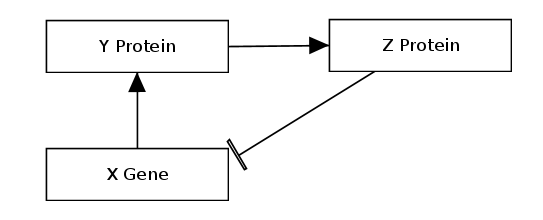
\includegraphics[width=\textwidth]{sketch.png}
	    \caption{
		One-Cell Model\\
	    The gene mRNA $X$ codes for protein $Y$ which, in turn, activates transcriptional inhibitor $Z$. The resulting model behaves as a three-variable oscillator.
	    }
	\end{subfigure}
	~
	\begin{subfigure}[b]{0.5\textwidth}
	    \begin{equation*}\frac{\delta X}{\delta t} = v_1 \frac{K_1^n}{K_1^n + Z^n} - v_2 \frac{X}{K_2 + X} \end{equation*}
	    \begin{equation*}\frac{\delta Y}{\delta t} = k_3 X - v_4 \frac{Y}{K_4 + Y}\end{equation*}
	    \begin{equation*}\frac{\delta Z}{\delta t} = k_5 Y - v_6 \frac{Z}{K_6 + Z}\end{equation*}

	    \captionsetup{labelformat=empty}
	    \caption{\\
	    \begin{tabular}{@{}>{$}l<{$}l @{\hskip 0.2cm} | @{\hskip 0.2cm} @{}>{$}l<{$}l@{}}
		v_1 & translation rate of $X$ & K_1 & Michaelis constant of $X$ \\
		v_2 & degradation rate of $X$ & K_4 & Michaelis constant of $Y$ \\
		v_4 & degradation rate of $Y$ & K_6 & Michaelis constant of $Z$\\
		v_6 & degradation rate of $Z$ &&\\
		k_3 & transcription rate of $X$ && \\
		k_5 & transcription rate of $Z$ &&\\
	    \end{tabular}
	    }
	\end{subfigure}
    \end{figure*}

    \begin{figure*}[!h]
	\begin{subfigure}[b]{0.5\textwidth}
	    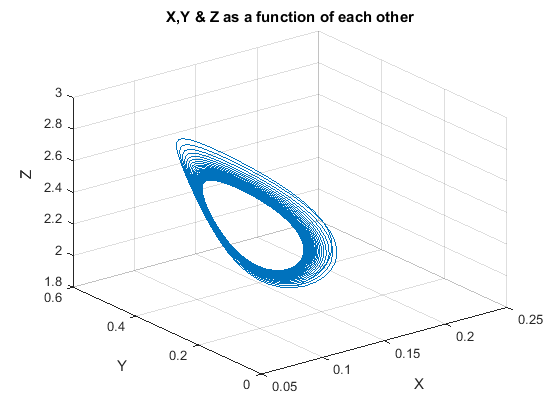
\includegraphics[width=\textwidth]{"../Miniprojet 2.0/Part A/A11.png}
	    \caption{Trajectories\\
	    The limit cycle is reached as the variations of $X(t)$, $Y(t)$ and $Z(t)$ become fixed : The trajectories converge, non-lineary (the distance between similar trajectories aren't regular) towards an ellipse (where the blue stripes accumulate)}
	\end{subfigure}
	~
	\begin{subfigure}[b]{0.5\textwidth}
	    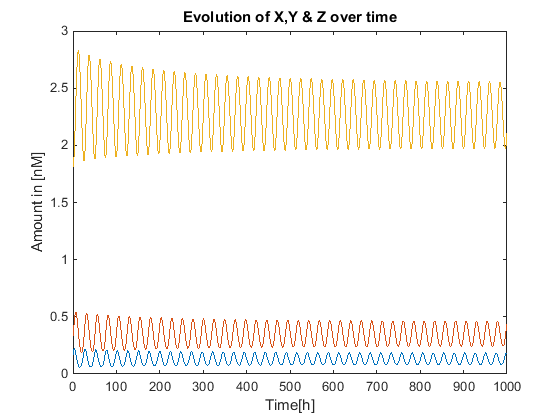
\includegraphics[width=\textwidth]{"../Miniprojet 2.0/Part A/A12.png}
	    \caption{Frequency spectrum \\
	    The amplitude of the three variations stabilize after a few hundred hours. The signal are not in phase but have the same, regular, frequencies.}
	\end{subfigure}
	\caption{\\Trajectories of $X(t)$, $Y(t)$ and $Z(t)$ with initial conditions : $X_0 = 0.16$, $Y_0 = 0.33 $, $Z_0 = 1.8$ [nM]\\ We observe on both graphs that $Z(t)$ has the bigger amplitude of variation whereas $X(t)$ and $Y(t)$ have small amplitudes. Additionaly, the convergence towards a single loop in (a) indicate that the frequencies of the signals are equal; this is illustrated as well in (b)
	}
    \end{figure*}

    \begin{figure*}
    \centering
	\begin{subfigure}[b]{0.32\textwidth}
	    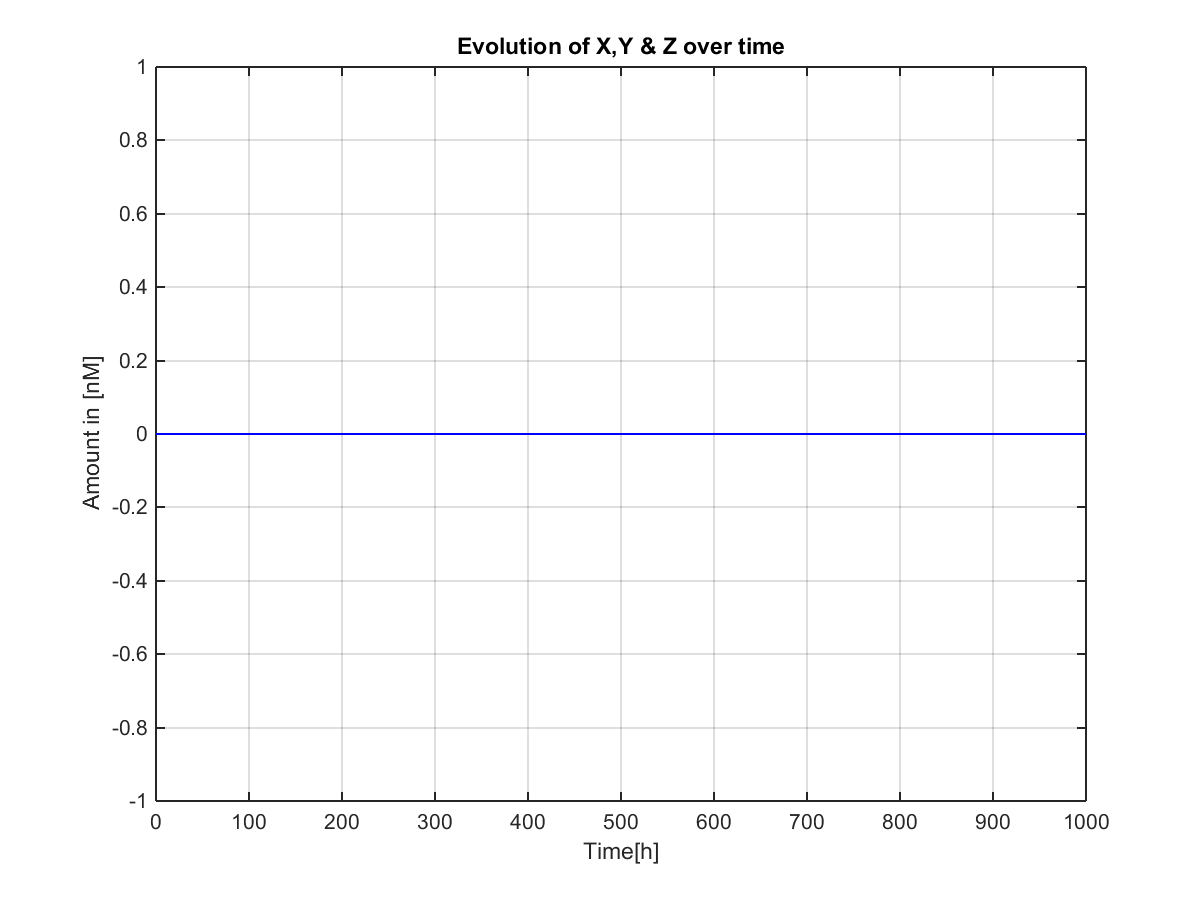
\includegraphics[width=\textwidth]{"../Miniprojet 2.0/Part A/A_3_graphs/A-A0.png}
	    \caption{$v_1$ = 0 nM/h}
	    \end{subfigure}
	    ~ 
	    \begin{subfigure}[b]{0.32\textwidth}
	    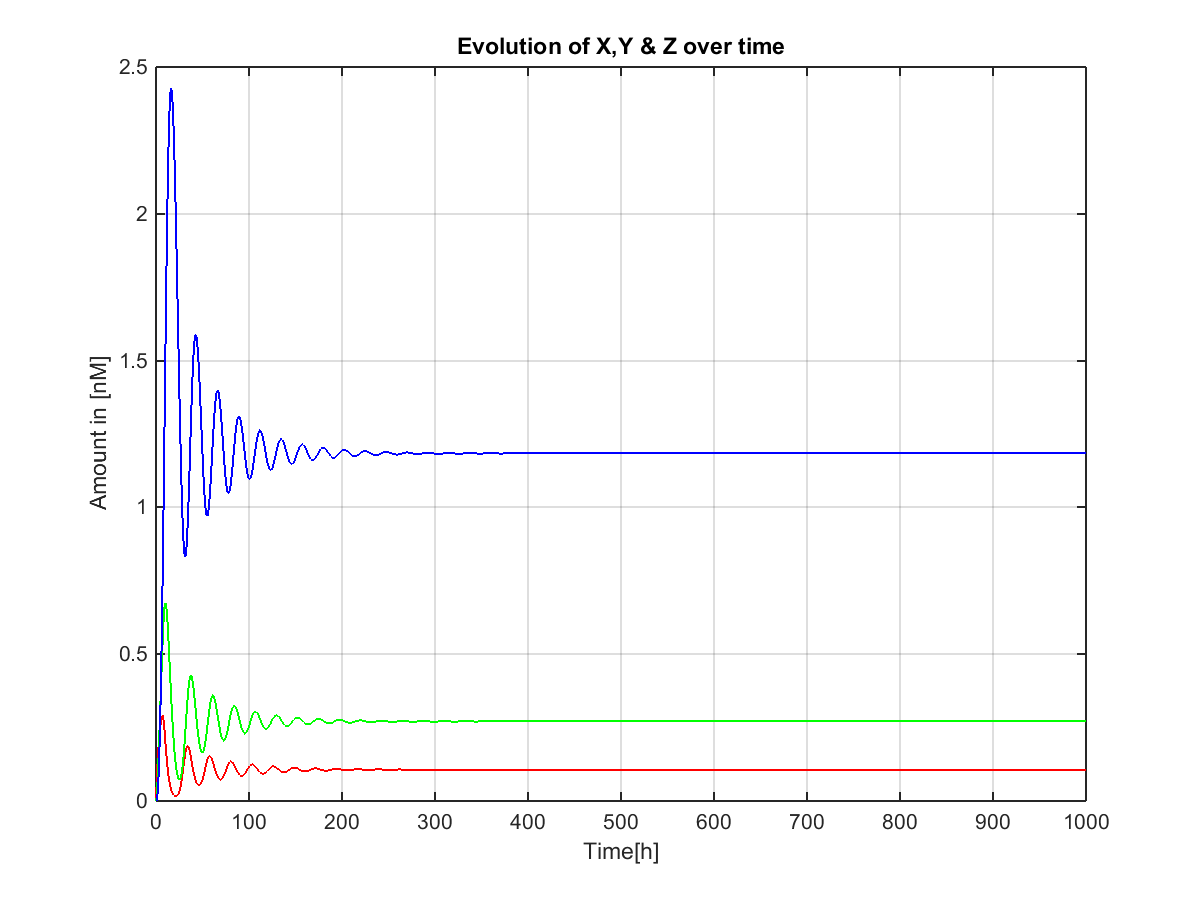
\includegraphics[width=\textwidth]{"../Miniprojet 2.0/Part A/A_3_graphs/A-A1.png}
	    \caption{$v_1$ = 1 nM/h}
	    \end{subfigure}
	    ~ 
	\begin{subfigure}[b]{0.32\textwidth}
	    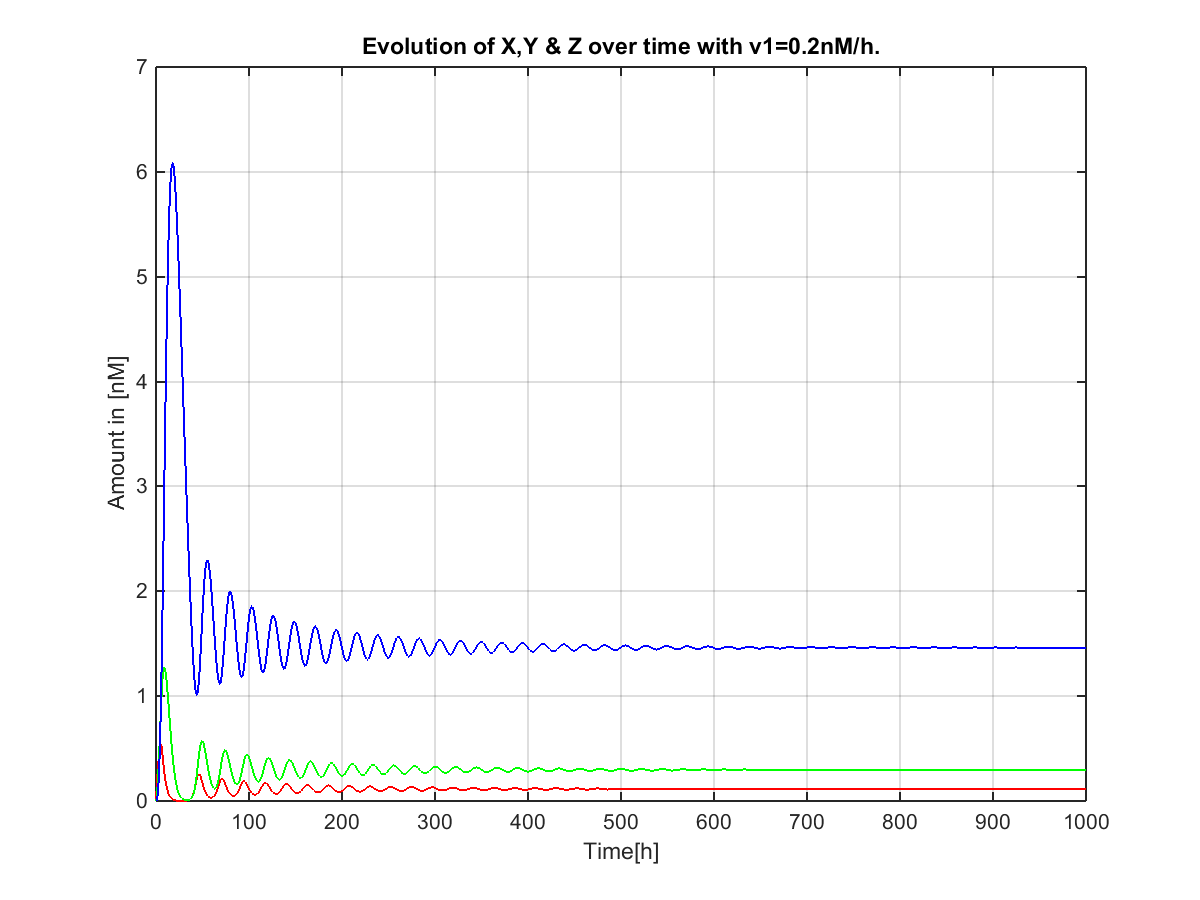
\includegraphics[width=\textwidth]{"../Miniprojet 2.0/Part A/A_3_graphs/A-A2.png}
	    \caption{$v_1$ = 2 nM/h}
	\end{subfigure}
	 
	\begin{subfigure}[b]{0.32\textwidth}
	    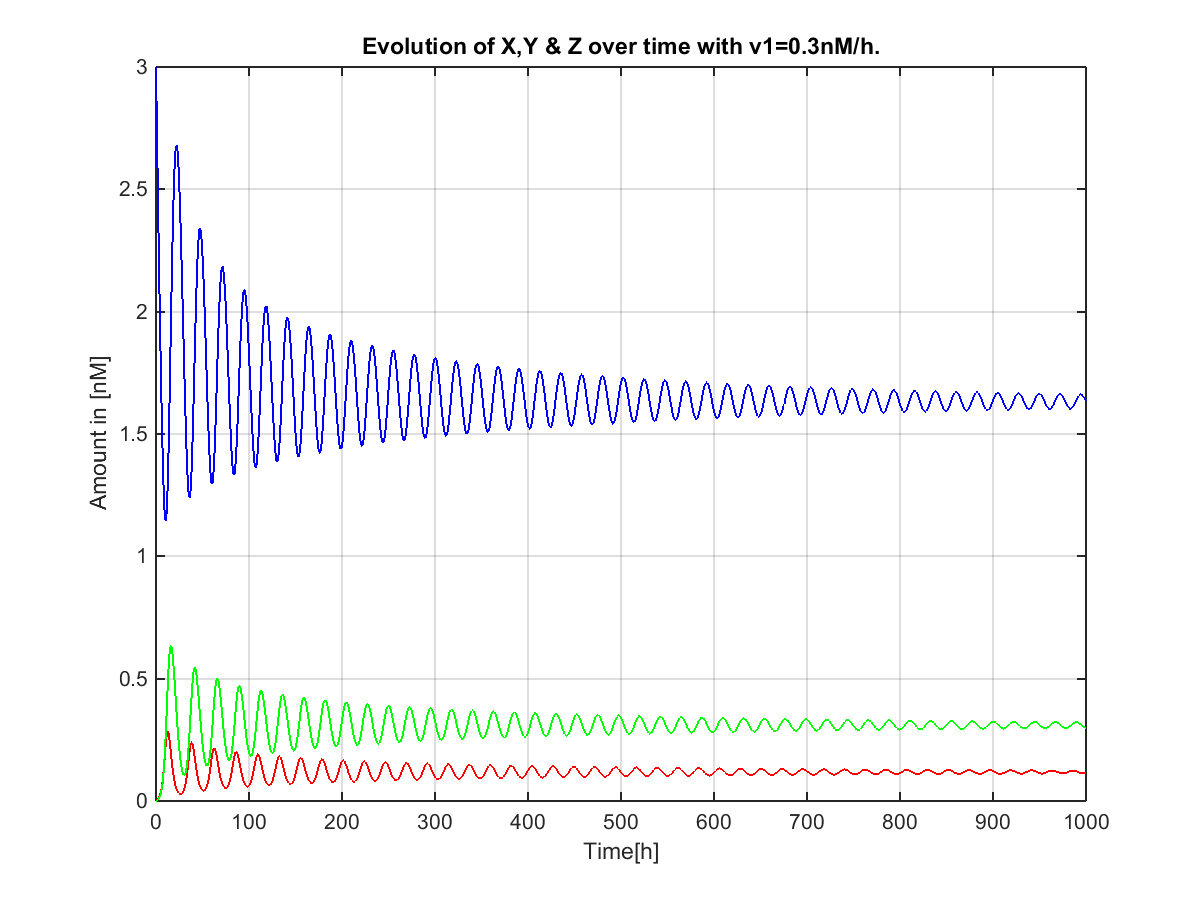
\includegraphics[width=\textwidth]{"../Miniprojet 2.0/Part A/A_3_graphs/A-A3.png}
	    \caption{$v_1$ = 3 nM/h}
	\end{subfigure}
	~ 
	\begin{subfigure}[b]{0.32\textwidth}
	    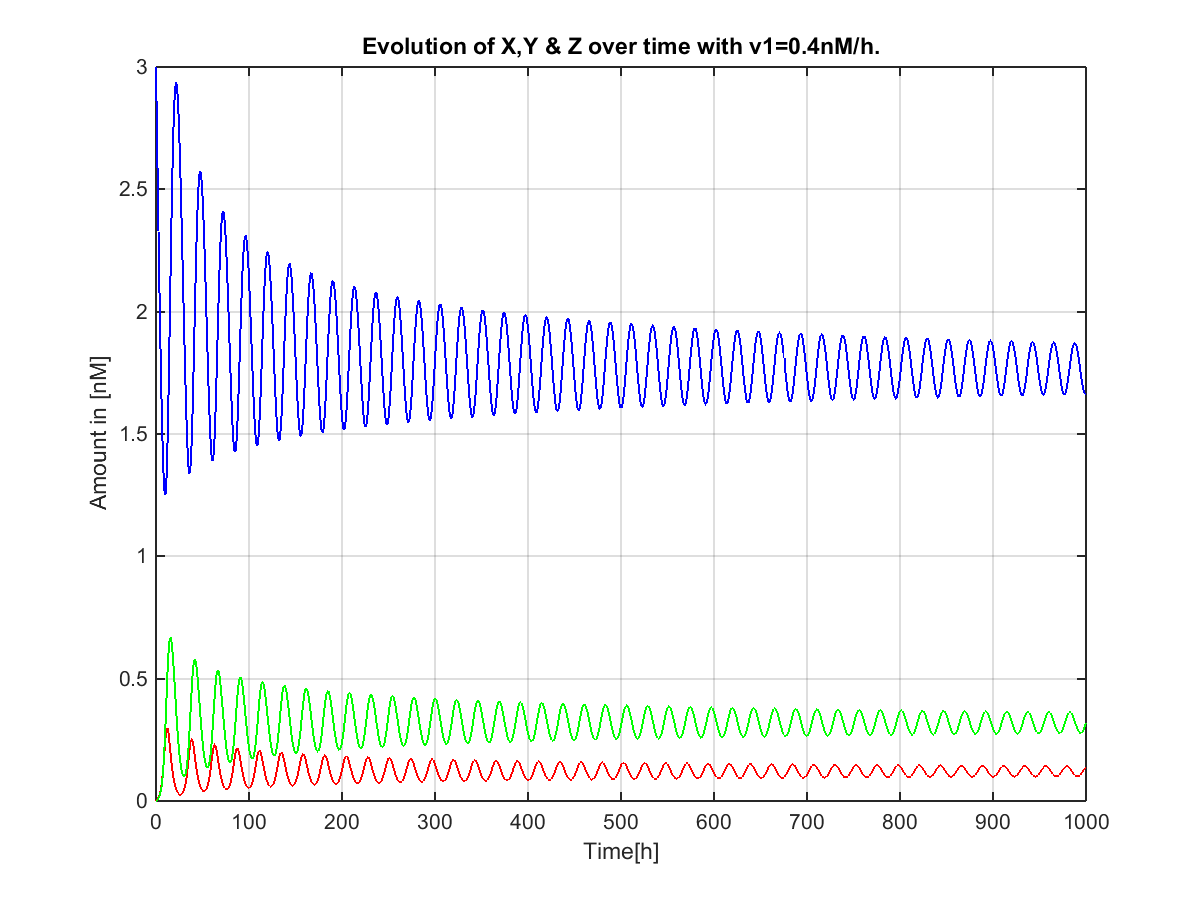
\includegraphics[width=\textwidth]{"../Miniprojet 2.0/Part A/A_3_graphs/A-A4.png}
	    \caption{$v_1$ = 4 nM/h}
	\end{subfigure}
	~
	\begin{subfigure}[b]{0.32\textwidth}
	    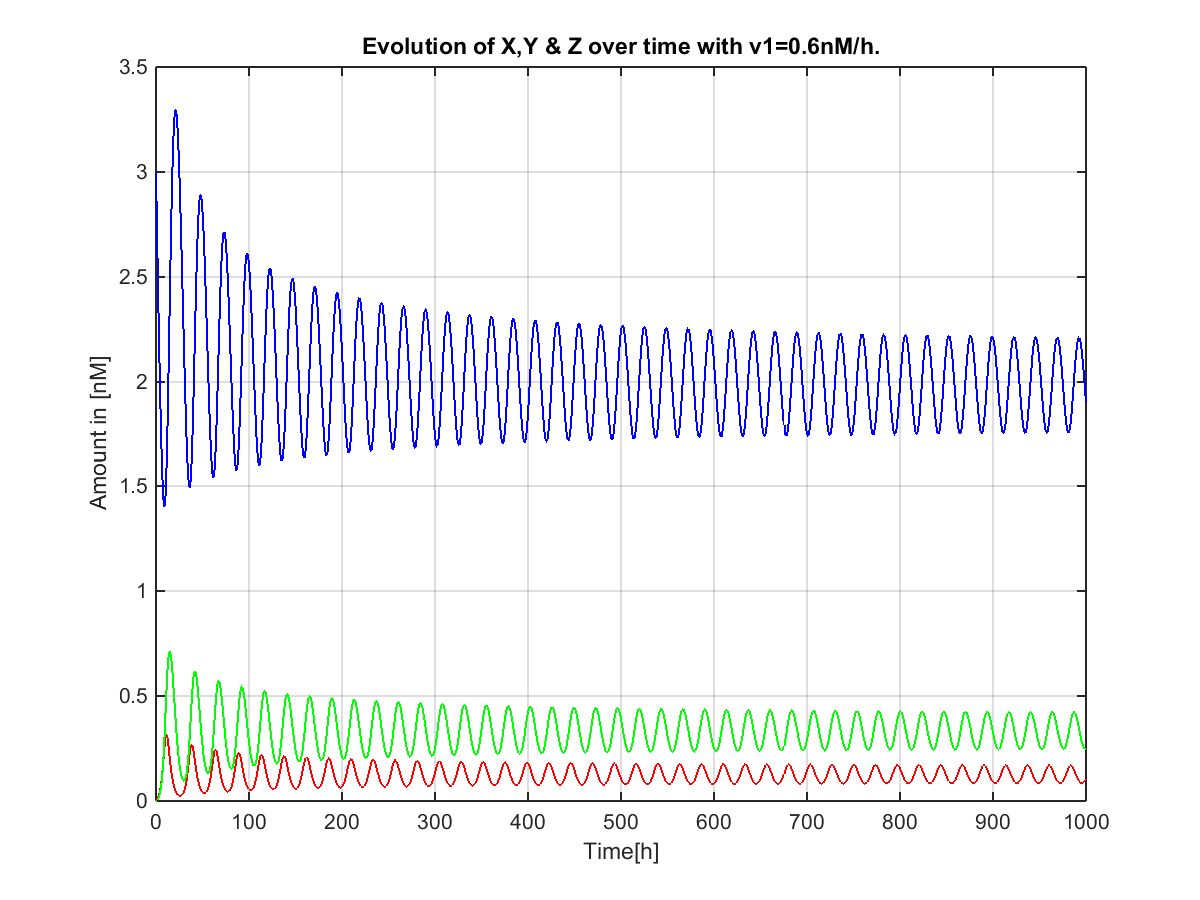
\includegraphics[width=\textwidth]{"../Miniprojet 2.0/Part A/A_3_graphs/A-A6.png}
	    \caption{$v_1$ = 6 nM/h}
	\end{subfigure}
	~ 
	\begin{subfigure}[b]{0.32\textwidth}
	    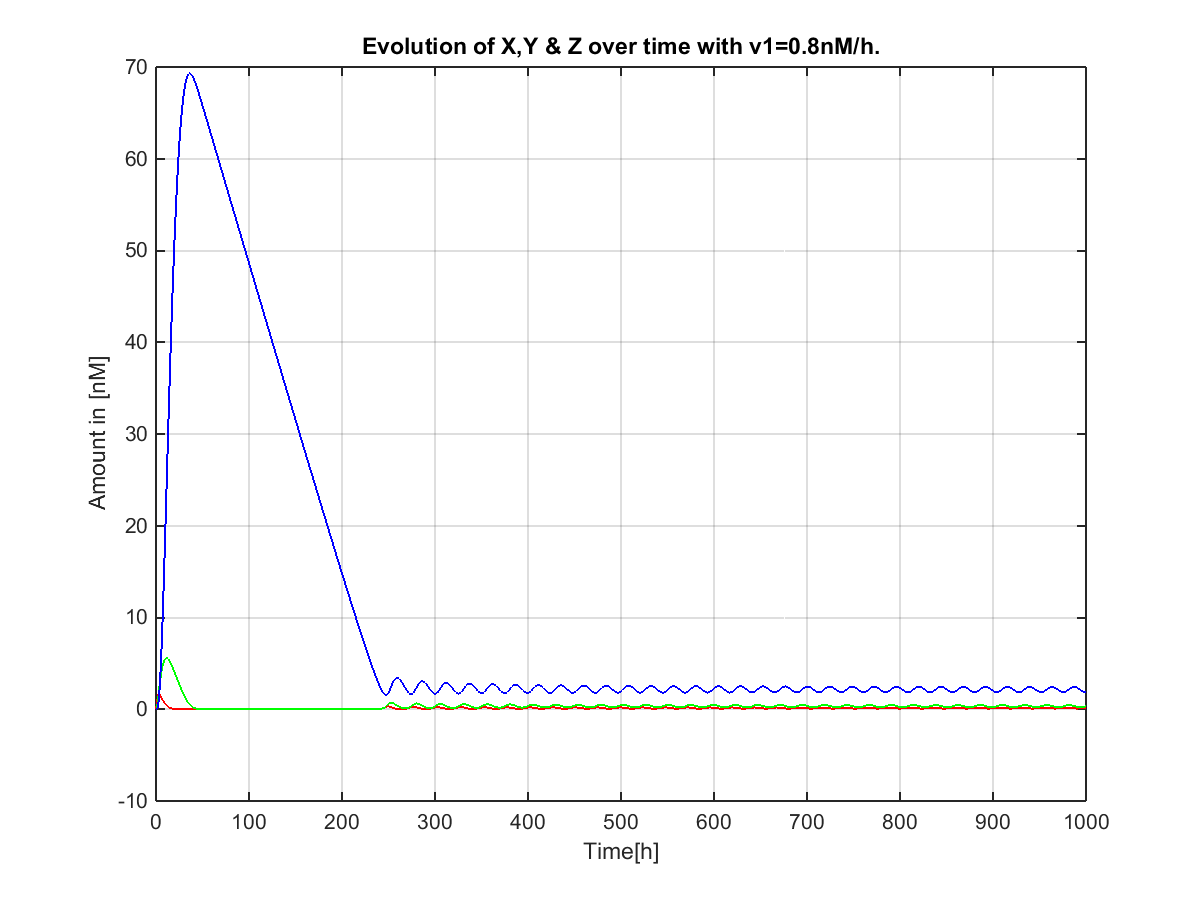
\includegraphics[width=\textwidth]{"../Miniprojet 2.0/Part A/A_3_graphs/A-A8.png}
	    \caption{$v_1$ = 8 nM/h}
	\end{subfigure}
	~
	\begin{subfigure}[b]{0.32\textwidth}
	    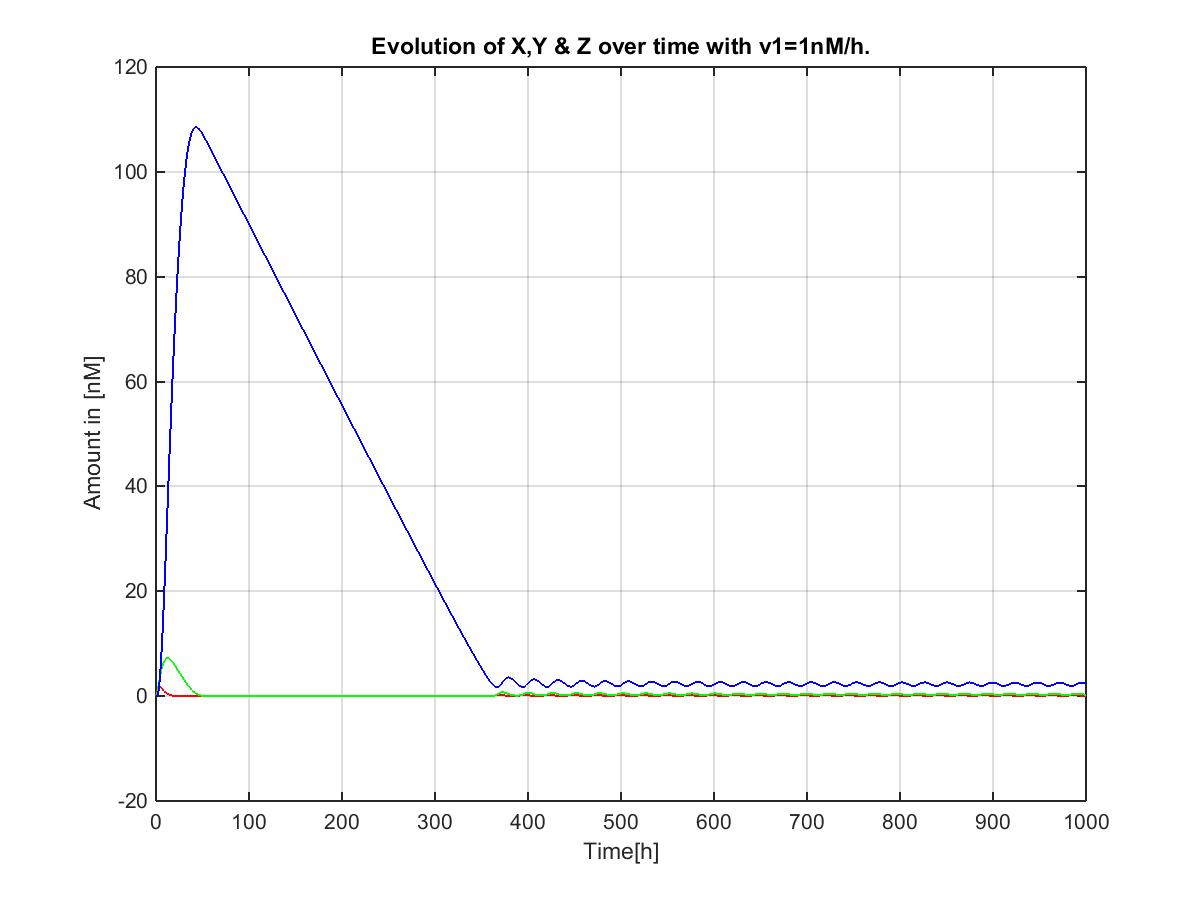
\includegraphics[width=\textwidth]{"../Miniprojet 2.0/Part A/A_3_graphs/A-A10.png}
	    \caption{$v_1$ = 10 nM/h}
	\end{subfigure}

	\caption{\green{$X(t)$}, \red{$Y(t)$} and \blue{$Z(t)$} with initial conditions $X_0 = 0.16$, $Y_0 = 0.33 $, $Z_0 = 1.8$ [nM]\\
	The first signal to fade is $Y(t)$ and its oscillatory stability predicts stability of the system. We also observe that the signals converge towards null or the limit cycle in a non-linear fashion. \red{At the opposite, it is rather difficult to predict the threshold value of $v_1$ using those plots ?}}
    \end{figure*}

    \begin{figure*}
	\centering
	    \begin{subfigure}[b]{0.43\textwidth}
		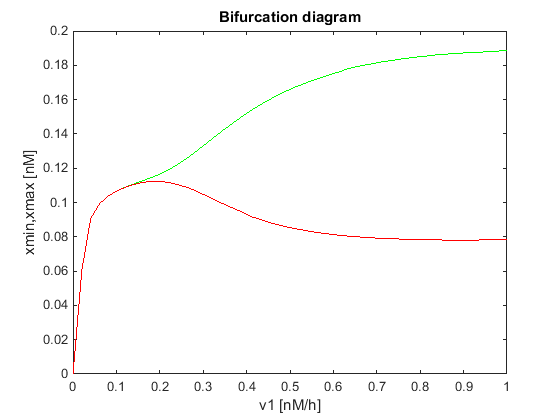
\includegraphics[width=\textwidth]{"../Miniprojet 2.0/Part A/Bifurcation.png}
		\caption{at $h_{max}=1000$ h}
	    \end{subfigure}
	     ~ 
	    \begin{subfigure}[b]{0.43\textwidth}
		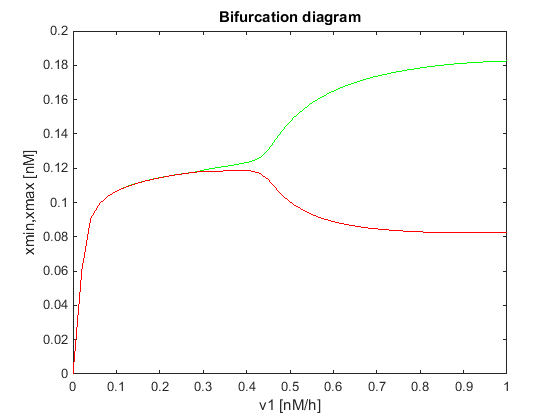
\includegraphics[width=\textwidth]{"../Miniprojet 2.0/Part A/Bifurcation10000.png}
		\caption{at $h_{max}=10~000$ h}
	    \end{subfigure}
	    \caption{Bifurcation Diagram : \red{$X_{min}$} and \green{$X_{max}$} plotted at time intervals $[9/10; 1]$ of $h_{max}$ \\
	    A limit cycle might be reached when $X_{min} \neq X_{max}$. However, the system needs to be run for enough time for the cycle to be reached, as the (a) suggests. (b) illustrates the non-linear convergence of the system; also the threshold for $v_1$ seems to be around 4.5}
    \end{figure*}

    \begin{figure*}
    \centering
	\begin{subfigure}[b]{0.32\textwidth}
	    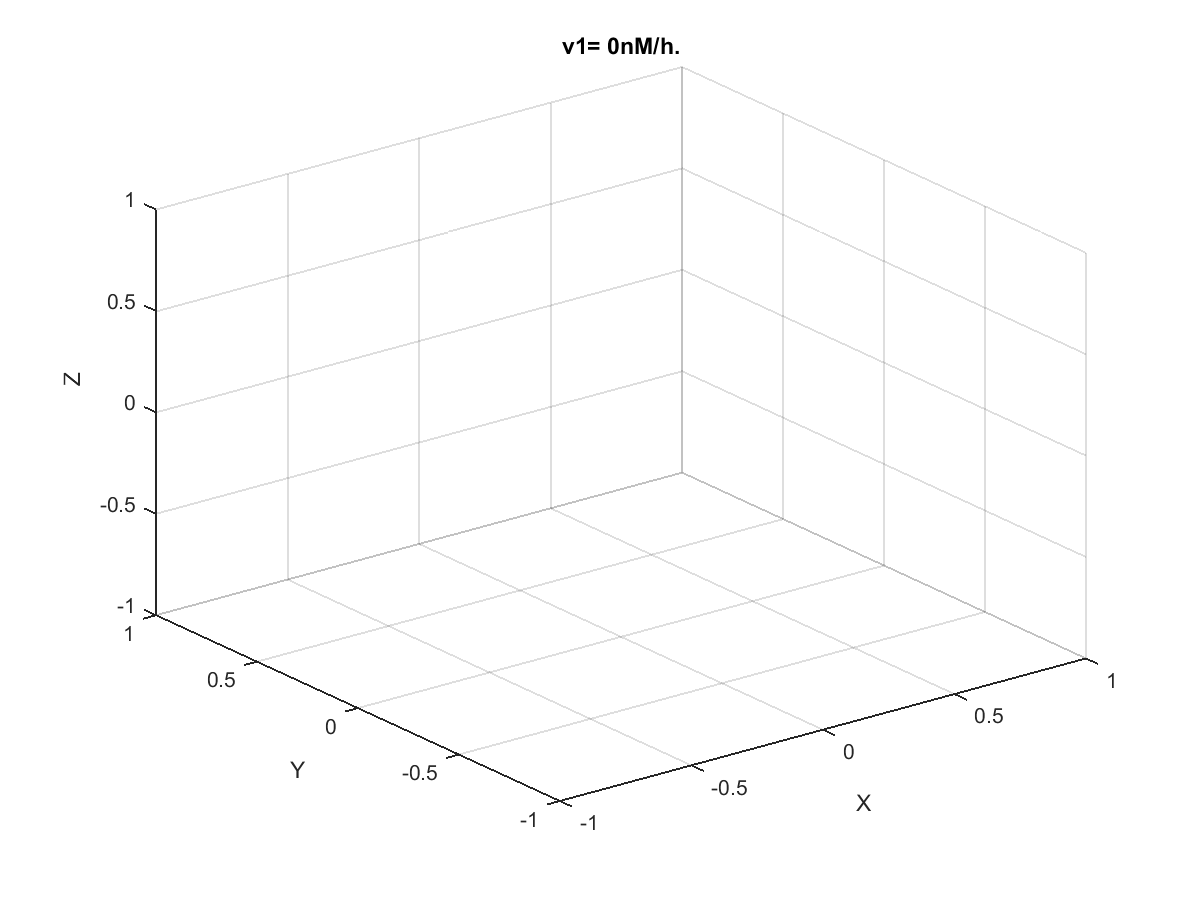
\includegraphics[width=\textwidth]{"../Miniprojet 2.0/Part A/A_3_graphs/A-AA0.png}
	    \caption{$v_1$ = 0 nM/h}
	\end{subfigure}
	~ 
	\begin{subfigure}[b]{0.32\textwidth}
	    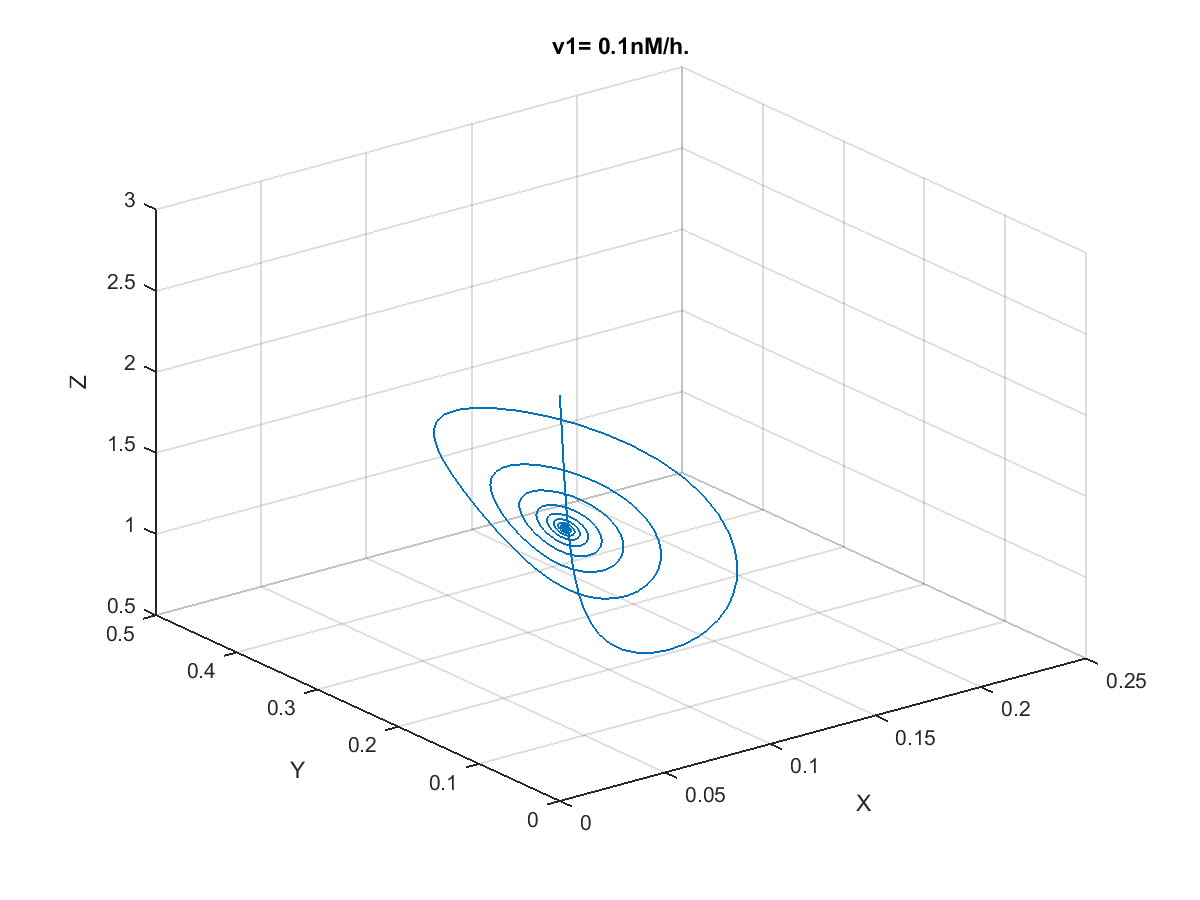
\includegraphics[width=\textwidth]{"../Miniprojet 2.0/Part A/A_3_graphs/A-AA1.png}
	    \caption{$v_1$ = 1 nM/h}
	\end{subfigure}
	~ 
	\begin{subfigure}[b]{0.32\textwidth}
	    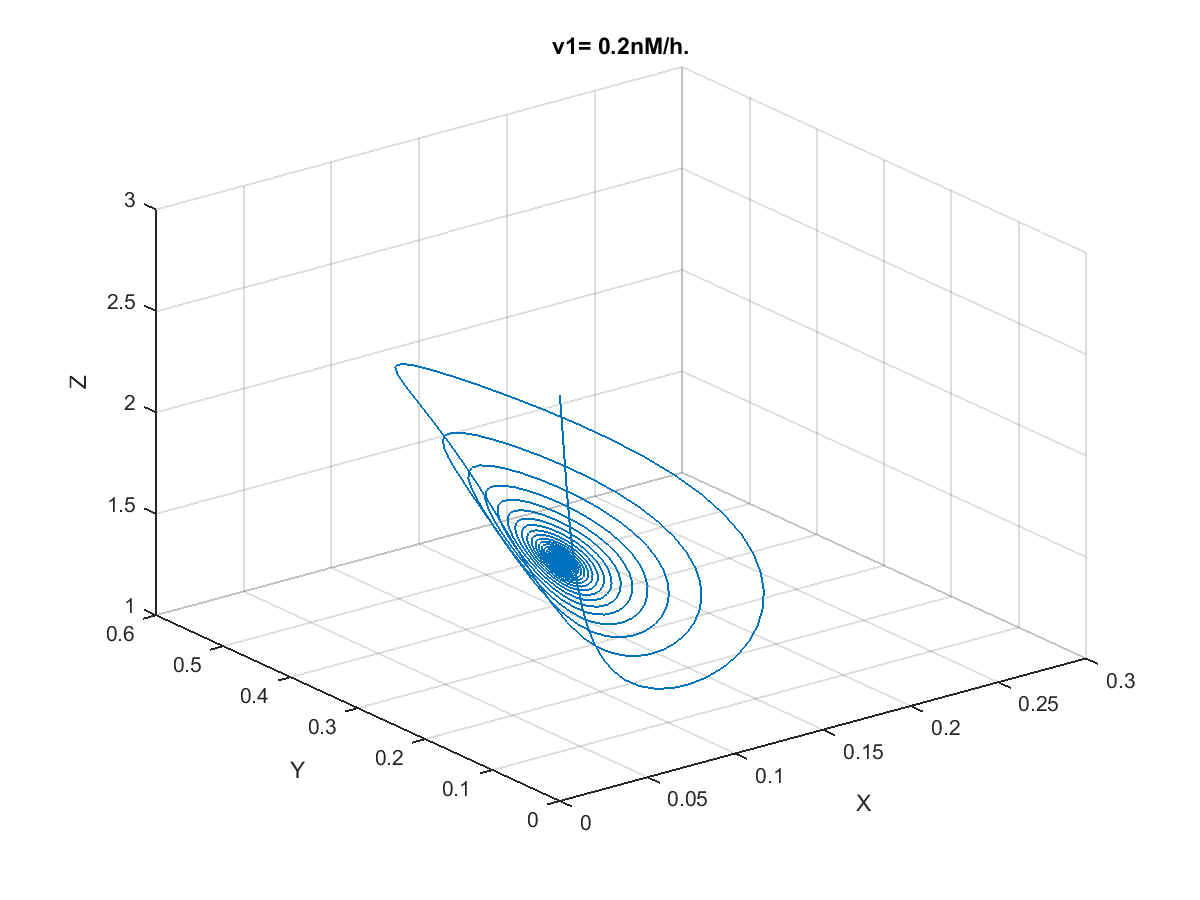
\includegraphics[width=\textwidth]{"../Miniprojet 2.0/Part A/A_3_graphs/A-AA2.png}
	    \caption{$v_1$ = 2 nM/h}
	\end{subfigure}
	 
	\begin{subfigure}[b]{0.32\textwidth}
	    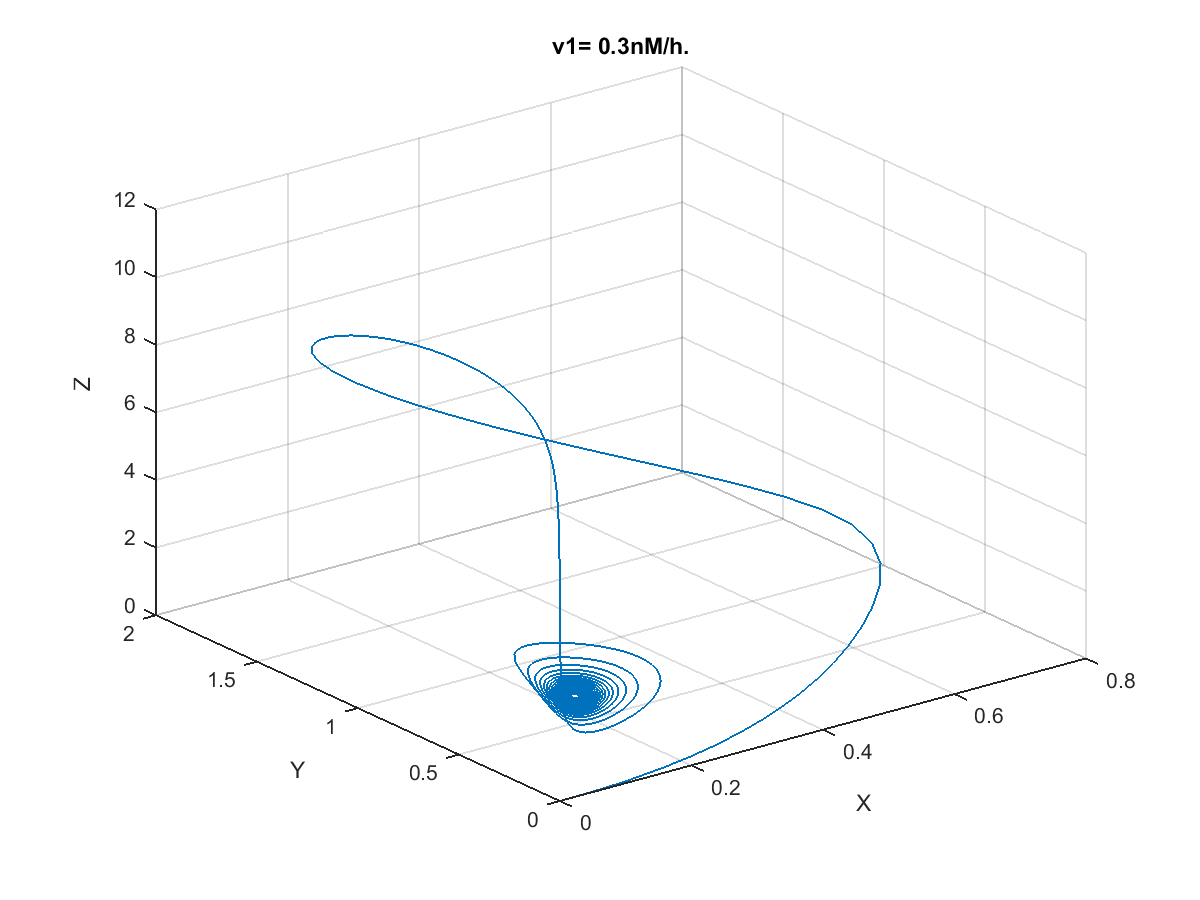
\includegraphics[width=\textwidth]{"../Miniprojet 2.0/Part A/A_3_graphs/A-AA3.png}
	    \caption{$v_1$ = 3 nM/h}
	\end{subfigure}
	~ 
	\begin{subfigure}[b]{0.32\textwidth}
	    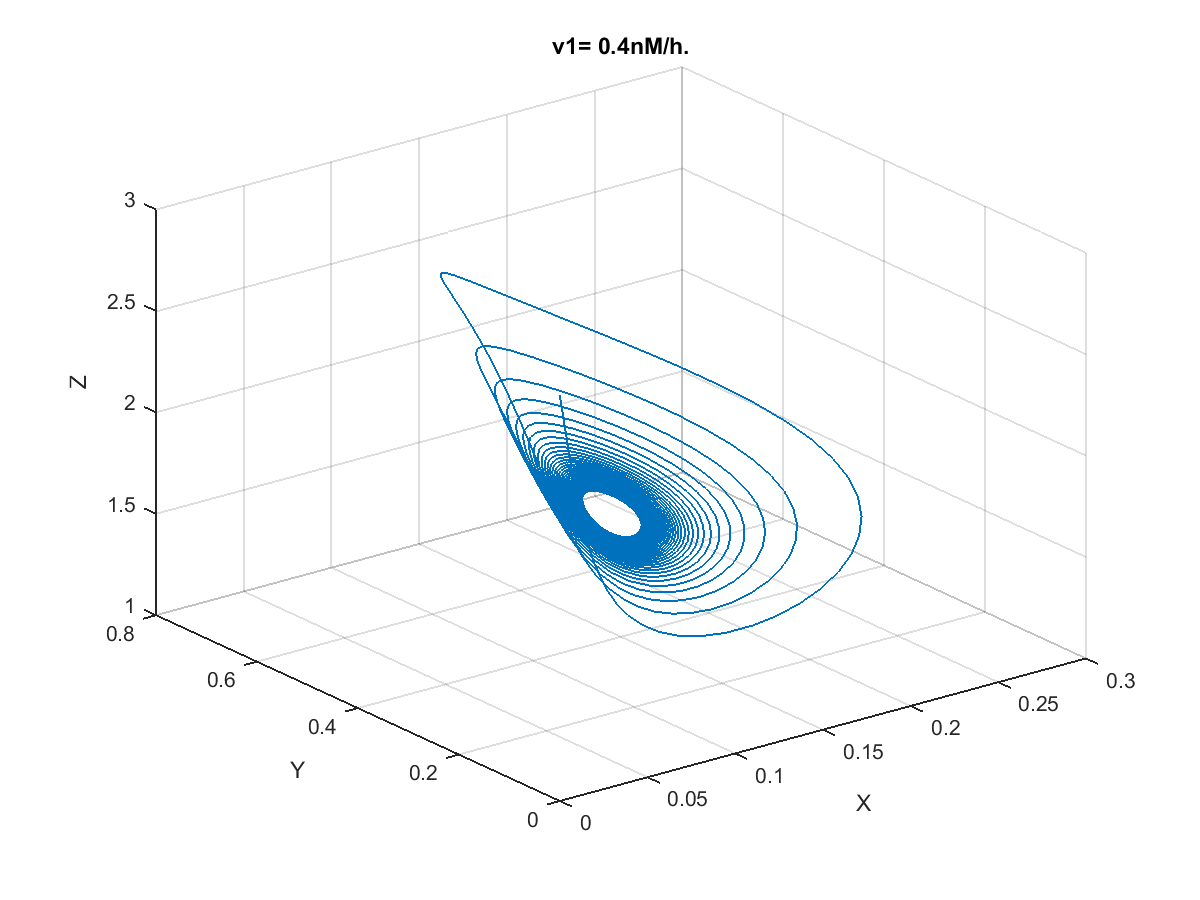
\includegraphics[width=\textwidth]{"../Miniprojet 2.0/Part A/A_3_graphs/A-AA4.png}
	    \caption{$v_1$ = 4 nM/h}
	\end{subfigure}
	~
	\begin{subfigure}[b]{0.32\textwidth}
	    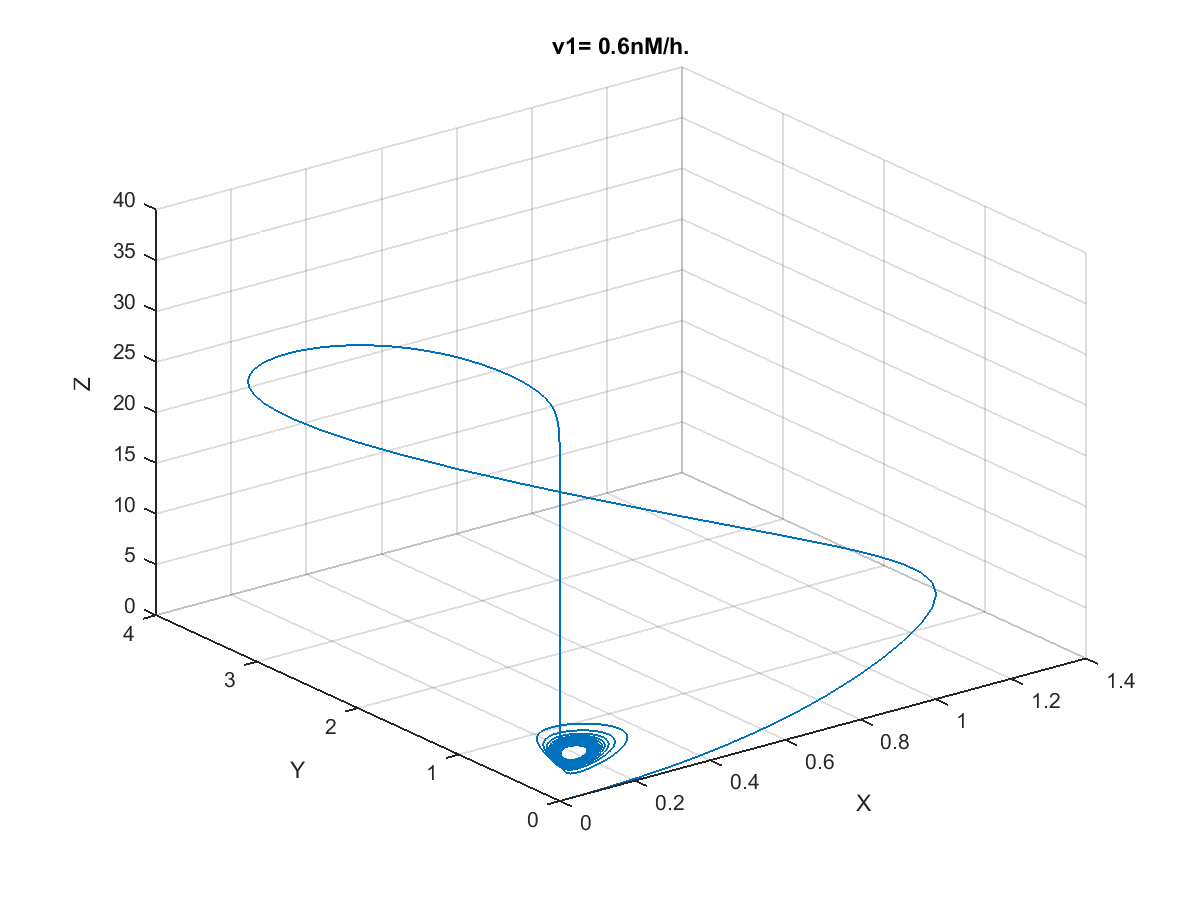
\includegraphics[width=\textwidth]{"../Miniprojet 2.0/Part A/A_3_graphs/A-AA6.png}
	    \caption{$v_1$ = 6 nM/h}
	\end{subfigure}
	~ 
	\begin{subfigure}[b]{0.32\textwidth}
	    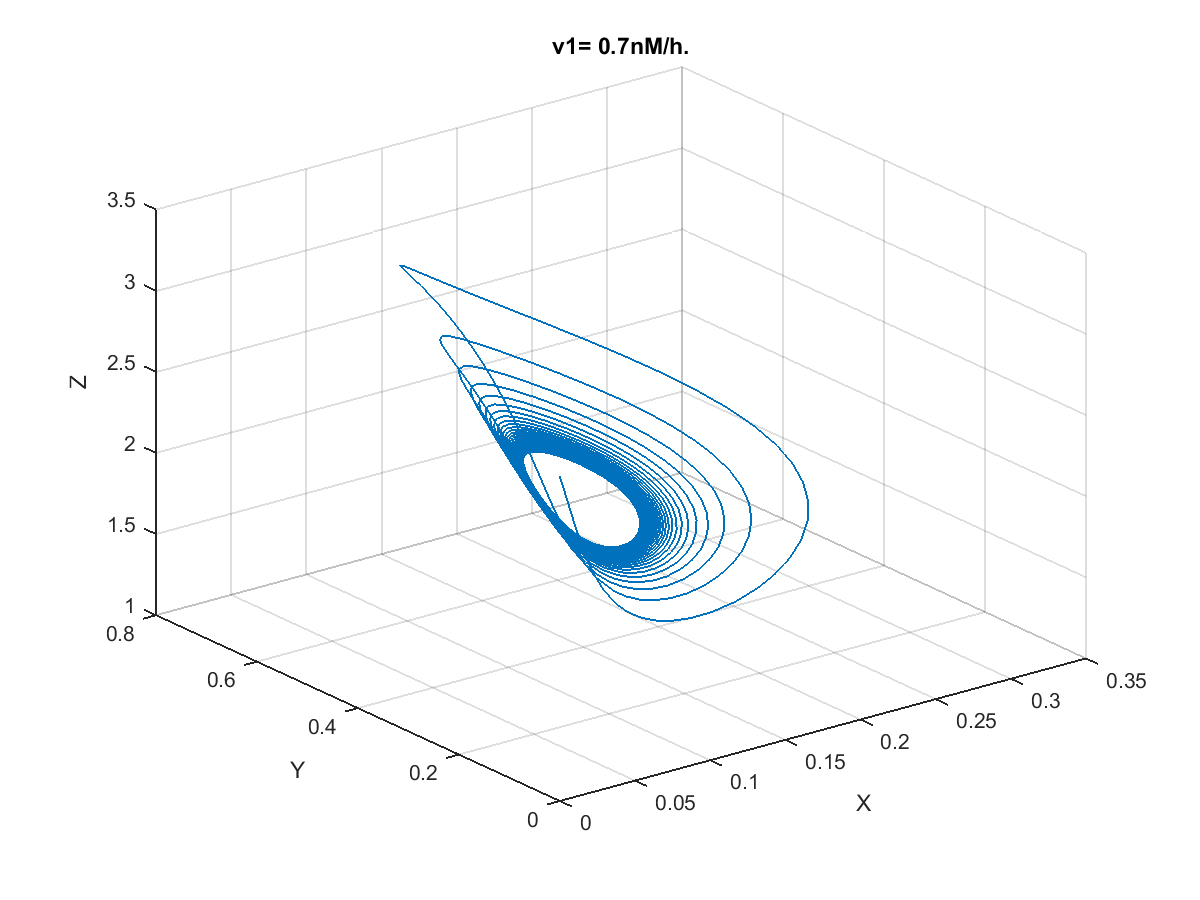
\includegraphics[width=\textwidth]{"../Miniprojet 2.0/Part A/A_3_graphs/A-AA7.png}
	    \caption{$v_1$ = 8 nM/h}
	\end{subfigure}
	~
	\begin{subfigure}[b]{0.32\textwidth}
	    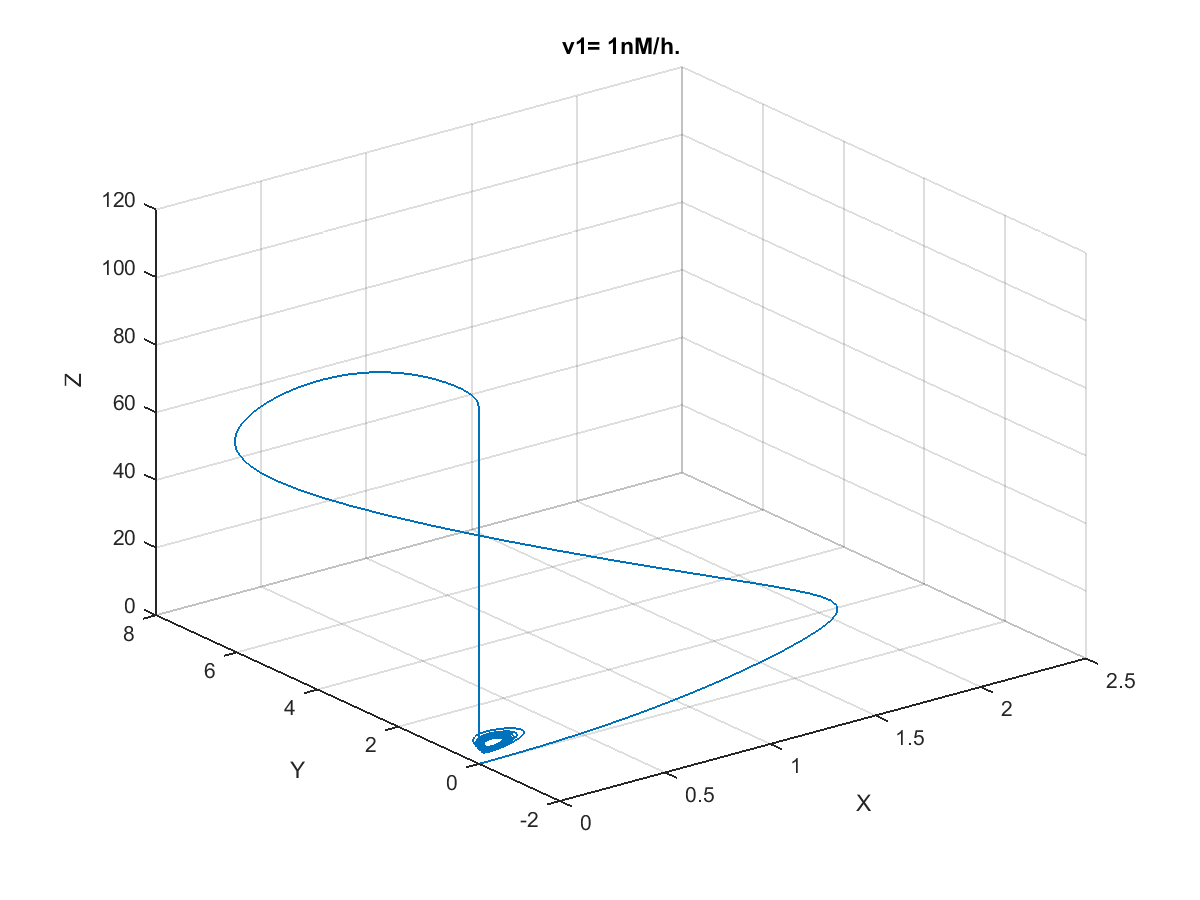
\includegraphics[width=\textwidth]{"../Miniprojet 2.0/Part A/A_3_graphs/A-AA10.png}
	    \caption{$v_1$ = 10 nM/h}
	\end{subfigure}
	
	\caption{Trajectories when varying $v_1$ with initial conditions $X_0 = 0.16$, $Y_0 = 0.33 $, $Z_0 = 1.8$ [nM]\\
	$v_1$ has to reach a certain value for $X(t)$ to be able to compensate its inhibition by $Z(t)$ and therefore for the system to reach a limit cycle. We observe that this value is slightly greater than 4nM/h, as the trajectories still converge to null in (e); there is an 'eye', even though it is smaller than in (f) and (g), since the timescale is not big enough to let the system dissipate completely.
	}
    \end{figure*}

    \begin{figure*}
	\centering
	    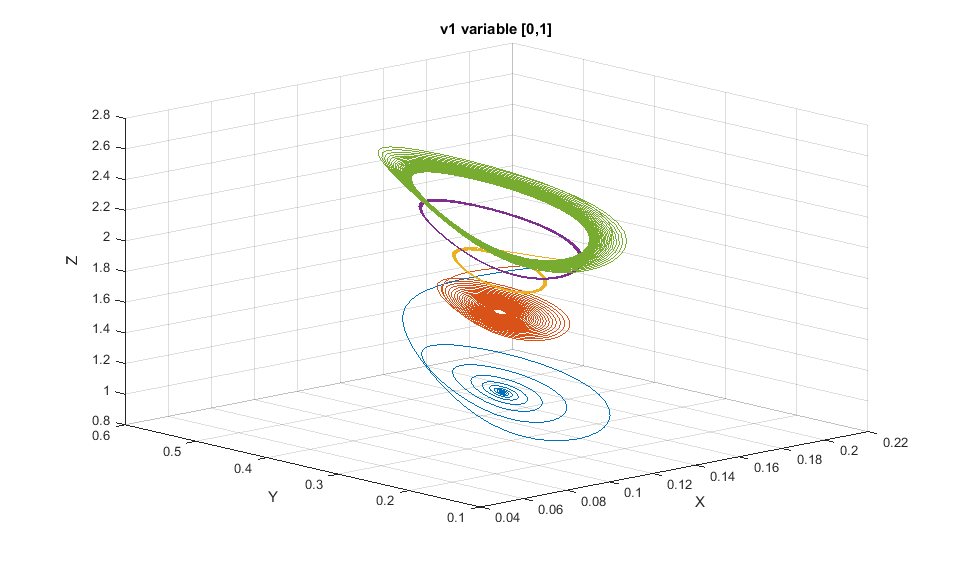
\includegraphics[width=0.5\textwidth]{"../Miniprojet 2.0/Part A/A2.png}
	    \caption{Superimposed trajectories at late timepoints with initial conditions $X_0 = 0.16$, $Y_0 = 0.33 $, $Z_0 = 1.8$ [nM] and $v_1$ = \cyan{0.1}/\red{0.3}/\orange{0.5}/\purple{0.7}/\fgreen{0.9} nM/h. We observe here that $Z(t)$ tends to reach greater concentration stability with increasing $v_1$.
	    }
    \end{figure*}

    \begin{figure*}[!htb] 		%oh my god this is so ugly pls don't look at me
	\captionsetup{labelformat=empty}
	\caption{\Huge{\textbf{Part B - Multiple Cells Model}}}
    \end{figure*}

    \begin{figure*}[!h]
	\begin{subfigure}[b]{0.5\textwidth}
	    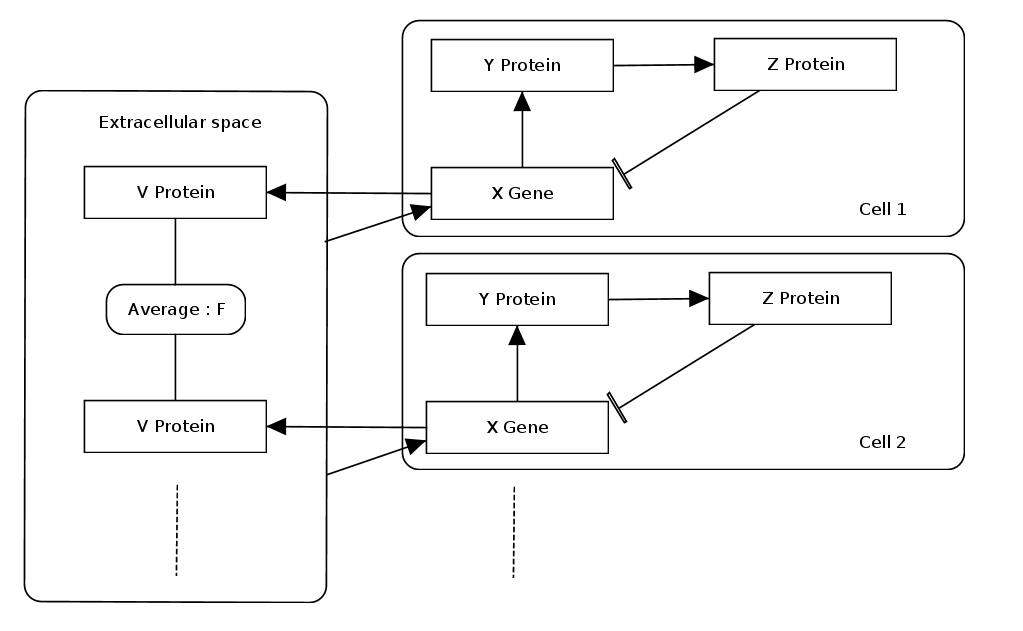
\includegraphics[width=\textwidth]{sketch2.png}
	    \caption{
		Multiple Cells Model\\
	    The gene $X$ codes for protein $Y$ which, in turn, activates transcriptional inhibitor $Z$. In addition, gene $X$ activates a positive feedback loop through the mean concentration of extracellular protein $V$
	    }
	\end{subfigure}
	~
	\begin{subfigure}[b]{0.5\textwidth}
	    \begin{equation*}\frac{\delta X}{\delta t} = v_1 \frac{K_1^n}{K_1^n + Z^n} - v_2 \frac{X}{K_2 + X} + v_c\frac{KF}{K_c + KF}\end{equation*}
	    \begin{equation*}\frac{\delta Y}{\delta t} = k_3 X - v_4 \frac{Y}{K_4 + Y}\end{equation*}
	    \begin{equation*}\frac{\delta Z}{\delta t} = k_5 Y - v_6 \frac{Z}{K_6 + Z}\end{equation*}
	    \begin{equation*}\frac{\delta V_i}{\delta t} = k_7 X_i - v_8 \frac{V_i}{K_8 + V_i}\end{equation*}
	    \begin{equation*}\text{where } F = \frac{1}{N}\sum_{i=1}^{N}V_i\end{equation*}

	    \captionsetup{labelformat=empty}
	    \caption{\\
	    \begin{tabular}{@{}>{$}l<{$}l @{\hskip 0.2cm} | @{\hskip 0.2cm} @{}>{$}l<{$}l@{}}
		v_1 & translation rate of $X$ & k_7 & transcription rate of $V$ \\
		v_2 & degradation rate of $X$ &	k_1 & transcription rate of $X$ \\
		v_4 & degradation rate of $Y$ & K_4 & Michaelis constant of $Y$ \\
		v_6 & degradation rate of $Z$ & K_6 & Michaelis constant of $Z$ \\
		v_8 & degradation rate of $V$ & K_8 & Michaelis constant of $V$ \\
		k_3 & transcription rate of $X$ & K & Coupling Constant \\
		k_5 & transcription rate of $Z$ && \\
	    \end{tabular}
	    }
	\end{subfigure}
    \end{figure*}


    \begin{figure*}
    \centering
	\begin{subfigure}[b]{0.32\textwidth}
	    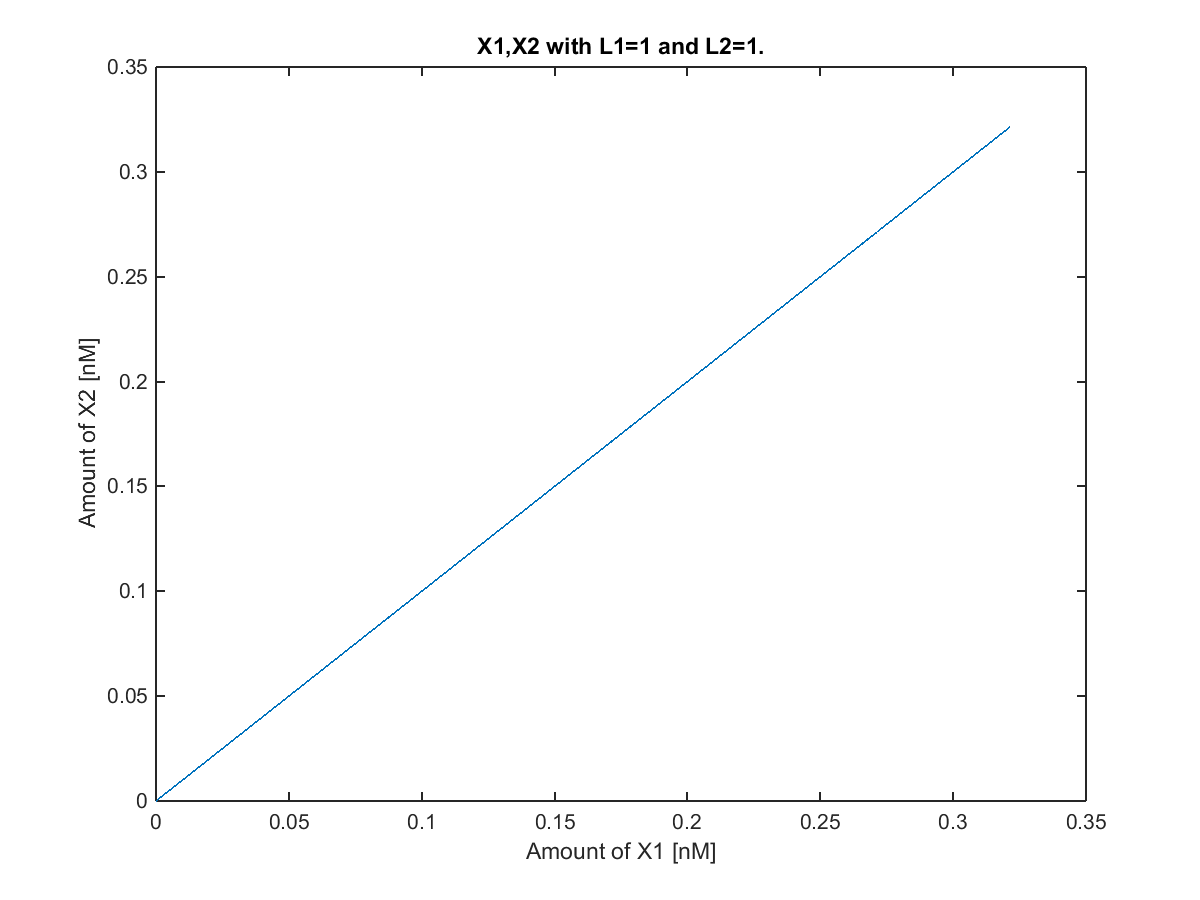
\includegraphics[width=\textwidth]{"../Miniprojet 2.0/Part B/B_2_graphs/B11.png}
	    \caption{$\lambda_1$ = 1, $\lambda_2$ = 1 [$h^{-1}$]}
	\end{subfigure}
	~ 
	\begin{subfigure}[b]{0.32\textwidth}
	    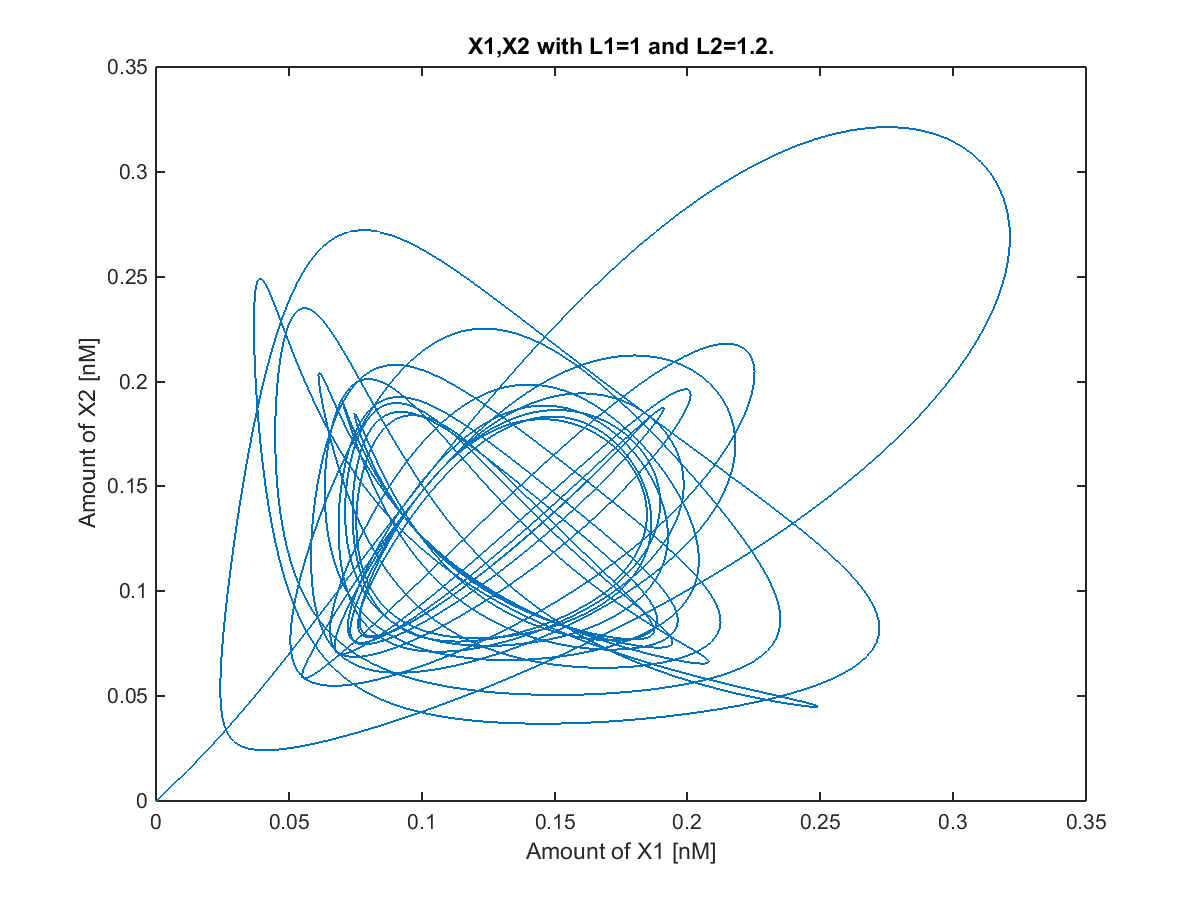
\includegraphics[width=\textwidth]{"../Miniprojet 2.0/Part B/B_2_graphs/B12.png}
	    \caption{$\lambda_1$ = 1, $\lambda_2$ = 1.2 [$h^{-1}$]}
	\end{subfigure}
	~ 
	\begin{subfigure}[b]{0.32\textwidth}
	    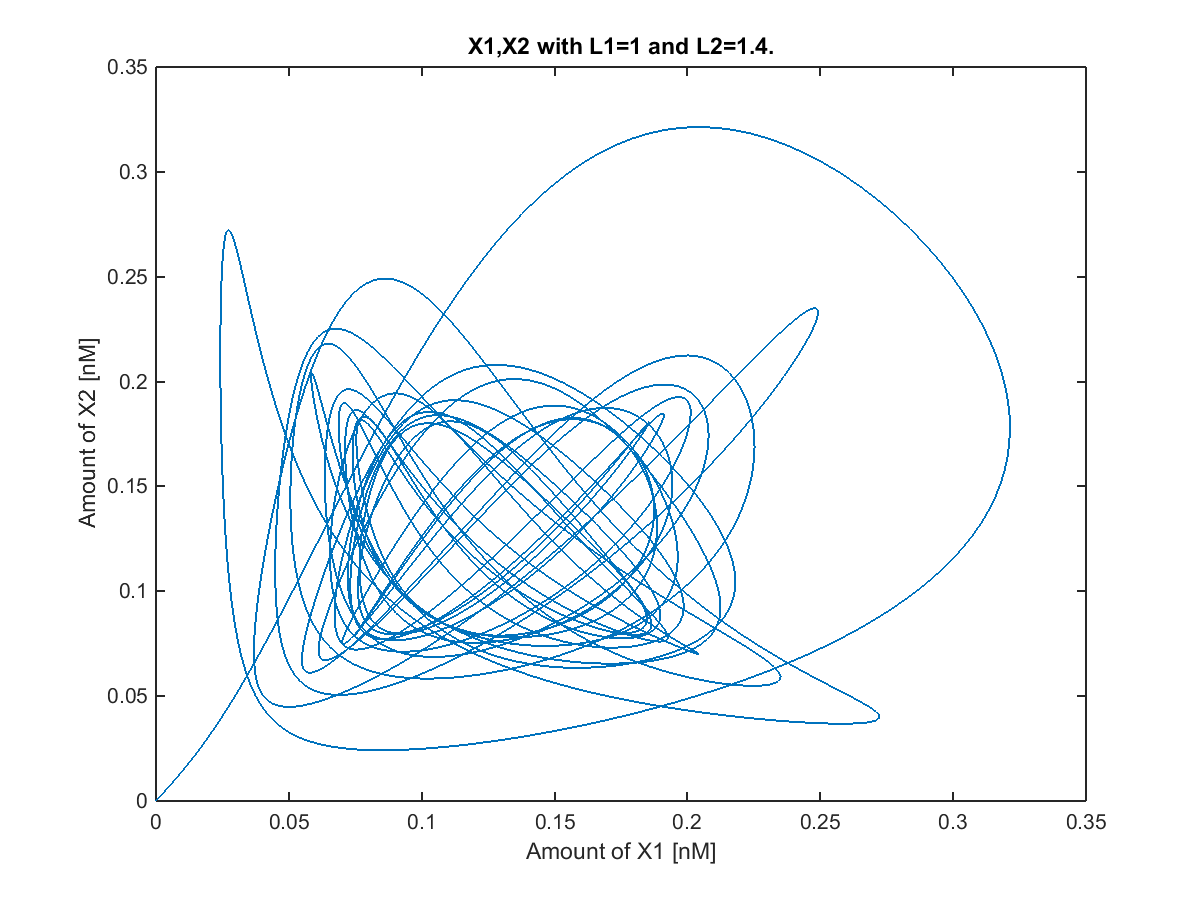
\includegraphics[width=\textwidth]{"../Miniprojet 2.0/Part B/B_2_graphs/B13.png}
	    \caption{$\lambda_1$ = 1, $\lambda_2$ = 1.4 [$h^{-1}$]}
	\end{subfigure}
	 
	\begin{subfigure}[b]{0.32\textwidth}
	    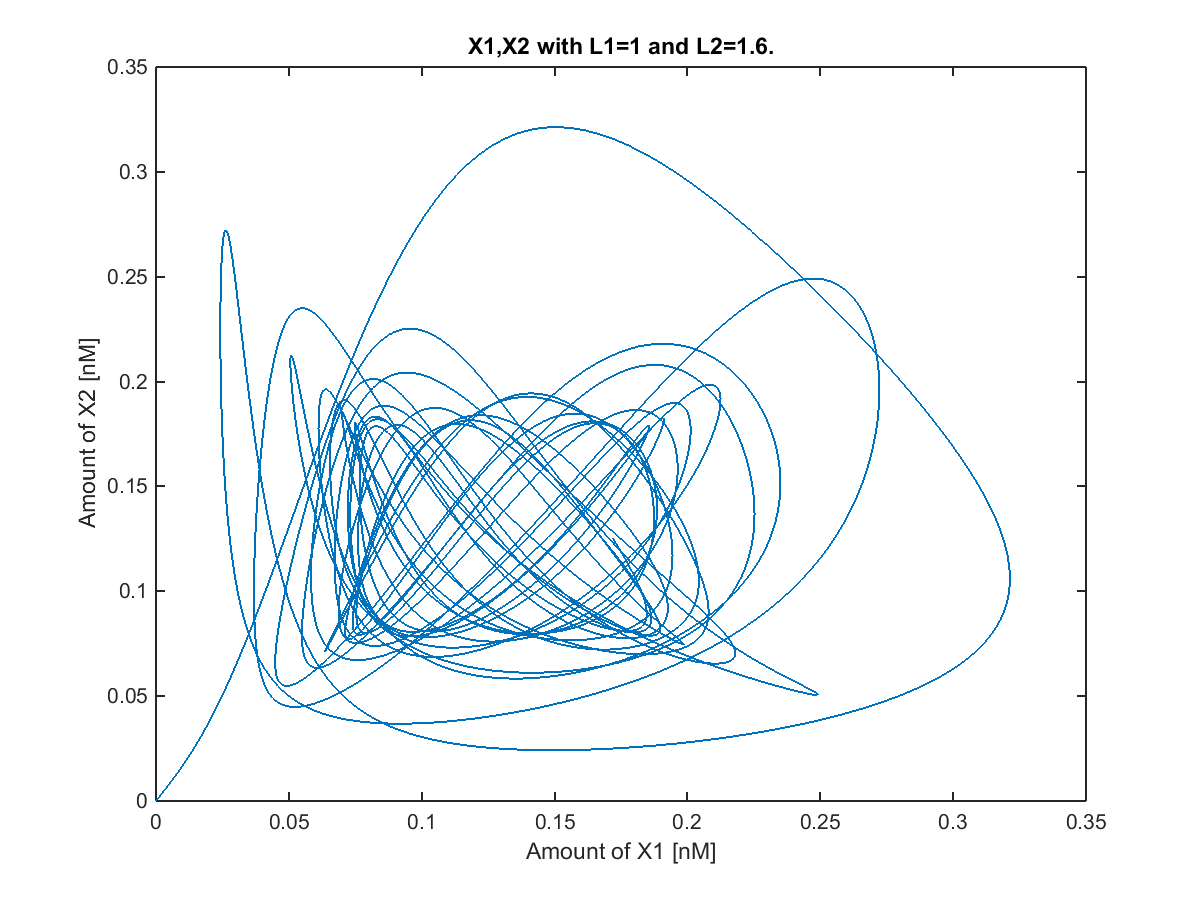
\includegraphics[width=\textwidth]{"../Miniprojet 2.0/Part B/B_2_graphs/B14.png}
	    \caption{$\lambda_1$ = 1, $\lambda_2$ = 1.6 [$h^{-1}$]}
	\end{subfigure}
	~ 
	\begin{subfigure}[b]{0.32\textwidth}
	    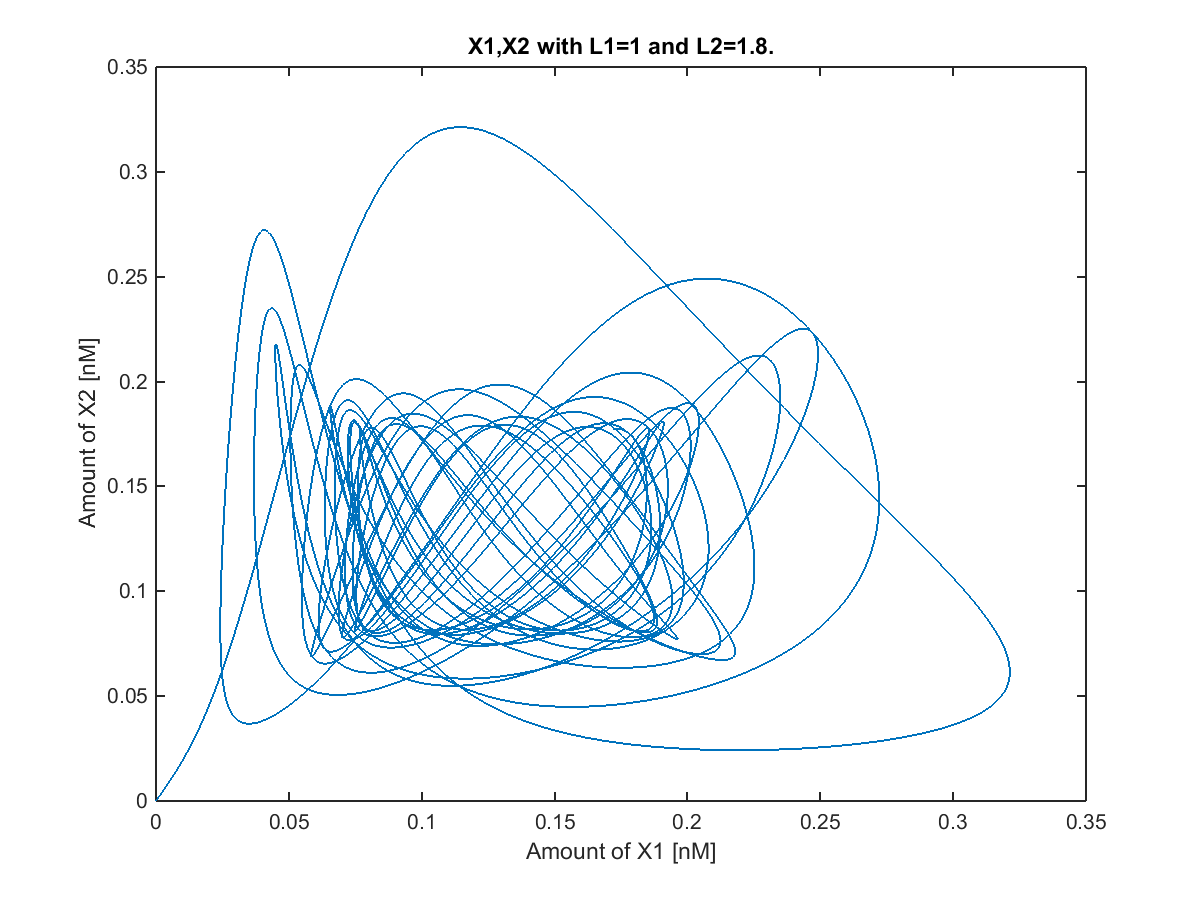
\includegraphics[width=\textwidth]{"../Miniprojet 2.0/Part B/B_2_graphs/B15.png}
	    \caption{$\lambda_1$ = 1, $\lambda_2$ = 1.8 [$h^{-1}$]}
	\end{subfigure}
	~ 
	\begin{subfigure}[b]{0.32\textwidth}
	    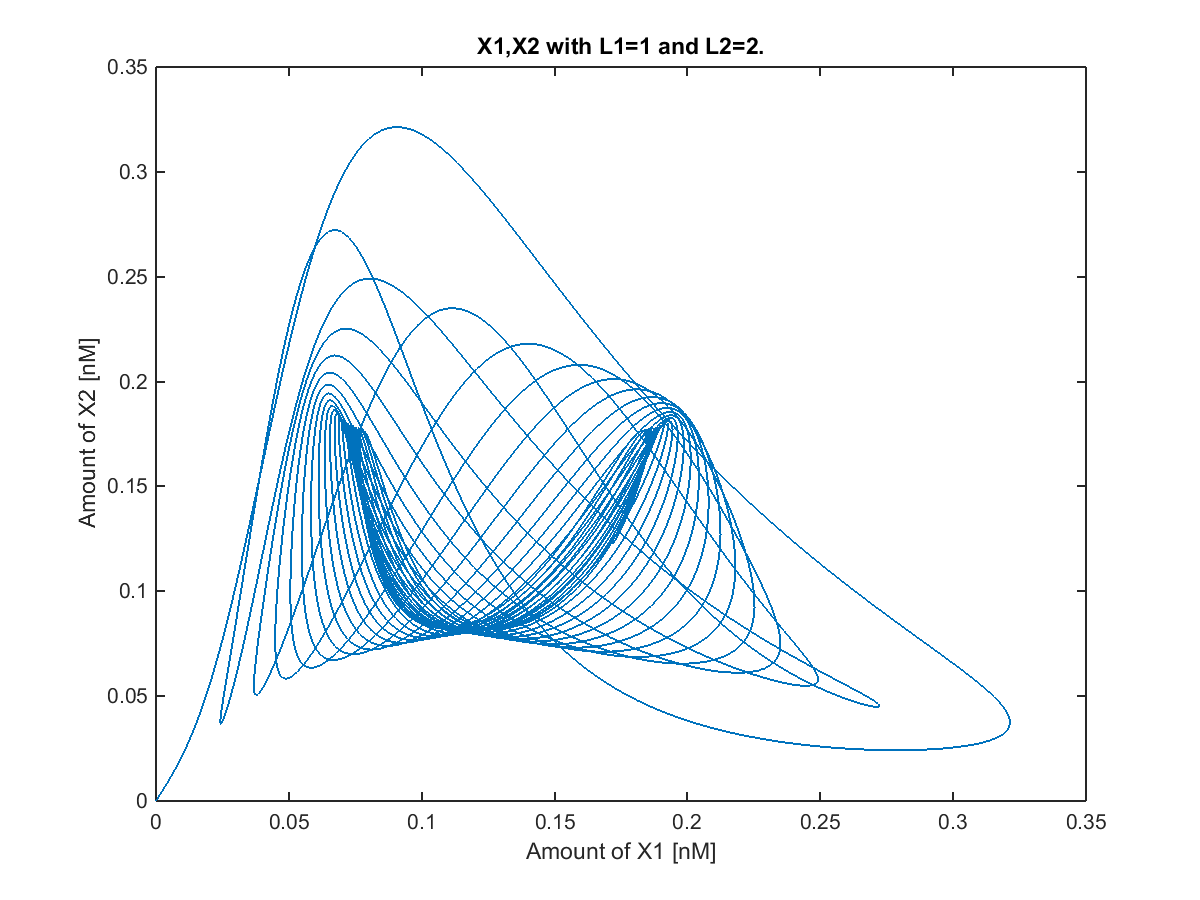
\includegraphics[width=\textwidth]{"../Miniprojet 2.0/Part B/B_2_graphs/B16.png}
	    \caption{$\lambda_1$ = 1, $\lambda_2$ = 2 [$h^{-1}$]}
	\end{subfigure}

	\caption{$X_1$ and $X_2$ trajectories with varying $\lambda_i$ in a two-cells Model\\
	\red{I don't really know what to say except 'wow it's cool' + square is max/min of Xs}}
    \end{figure*}

    \begin{figure*}
    \centering
	\begin{subfigure}[b]{0.32\textwidth}
	    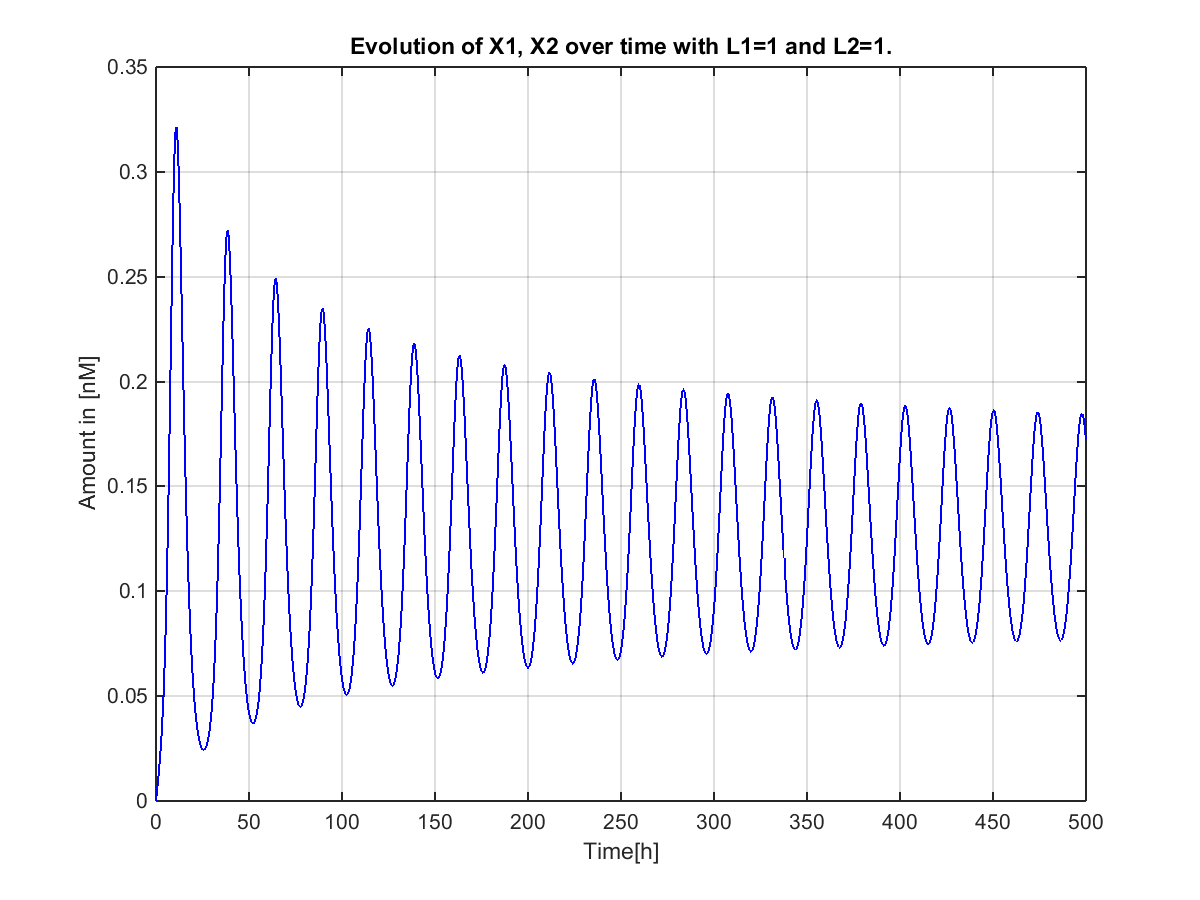
\includegraphics[width=\textwidth]{"../Miniprojet 2.0/Part B/B_2_graphs/B21.png}
	    \caption{$\lambda_1$ = 1, $\lambda_2$ = 1 [$h^{-1}$]}
	\end{subfigure}
	~ 
	\begin{subfigure}[b]{0.32\textwidth}
	    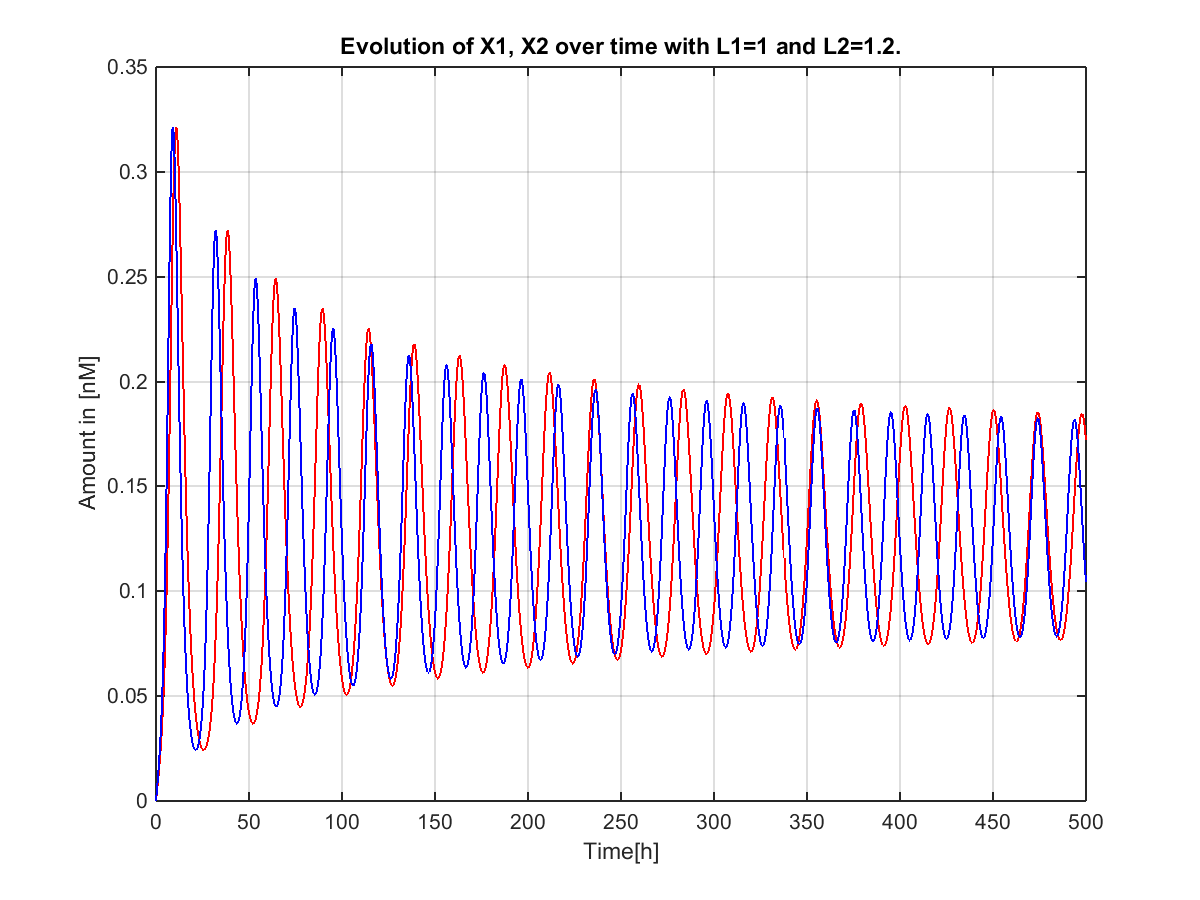
\includegraphics[width=\textwidth]{"../Miniprojet 2.0/Part B/B_2_graphs/B22.png}
	    \caption{$\lambda_1$ = 1, $\lambda_2$ = 1.2 [$h^{-1}$]}
	\end{subfigure}
	~ 
	\begin{subfigure}[b]{0.32\textwidth}
	    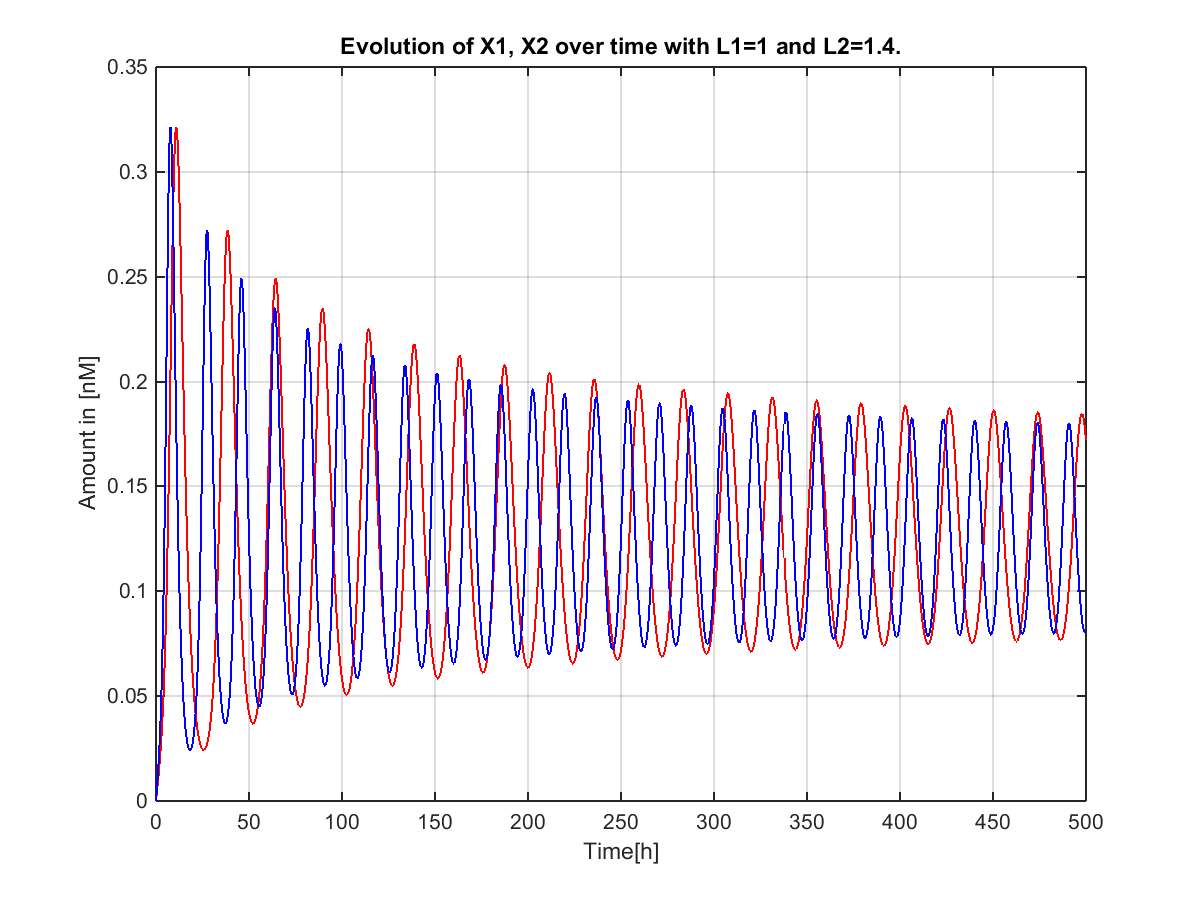
\includegraphics[width=\textwidth]{"../Miniprojet 2.0/Part B/B_2_graphs/B23.png}
	    \caption{$\lambda_1$ = 1, $\lambda_2$ = 1.4 [$h^{-1}$]}
	\end{subfigure}
	 
	\begin{subfigure}[b]{0.32\textwidth}
	    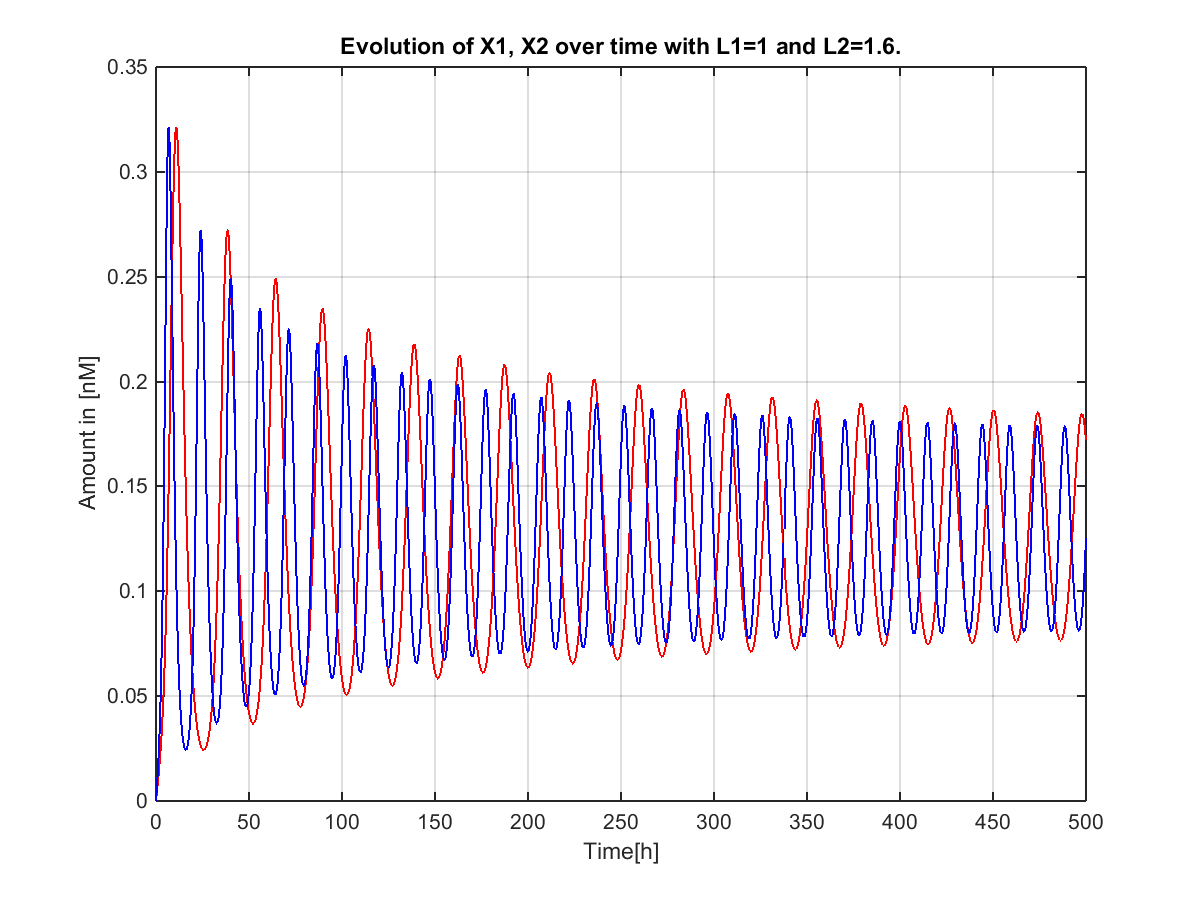
\includegraphics[width=\textwidth]{"../Miniprojet 2.0/Part B/B_2_graphs/B24.png}
	    \caption{$\lambda_1$ = 1, $\lambda_2$ = 1.6 [$h^{-1}$]}
	\end{subfigure}
	~ 
	\begin{subfigure}[b]{0.32\textwidth}
	    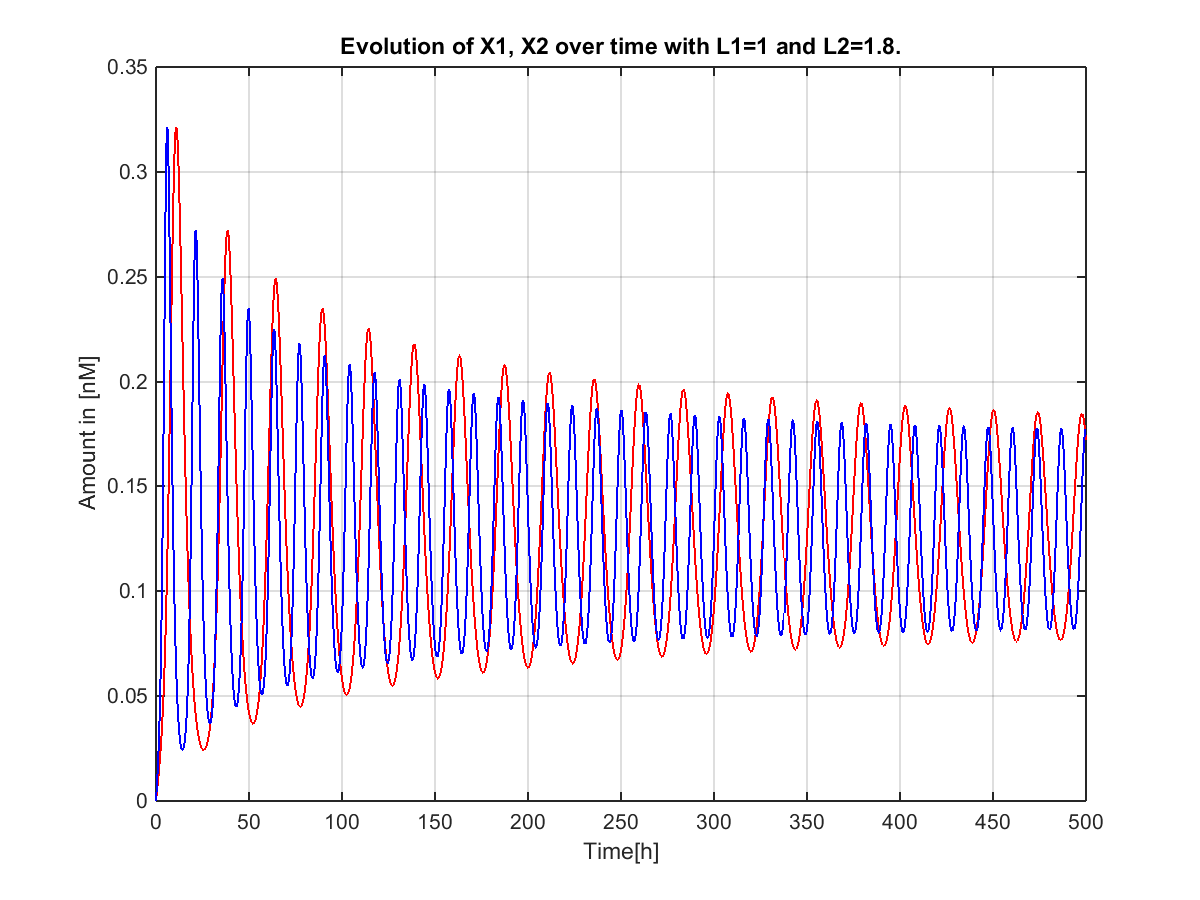
\includegraphics[width=\textwidth]{"../Miniprojet 2.0/Part B/B_2_graphs/B25.png}
	    \caption{$\lambda_1$ = 1, $\lambda_2$ = 1.8 [$h^{-1}$]}
	\end{subfigure}
	~ 
	\begin{subfigure}[b]{0.32\textwidth}
	    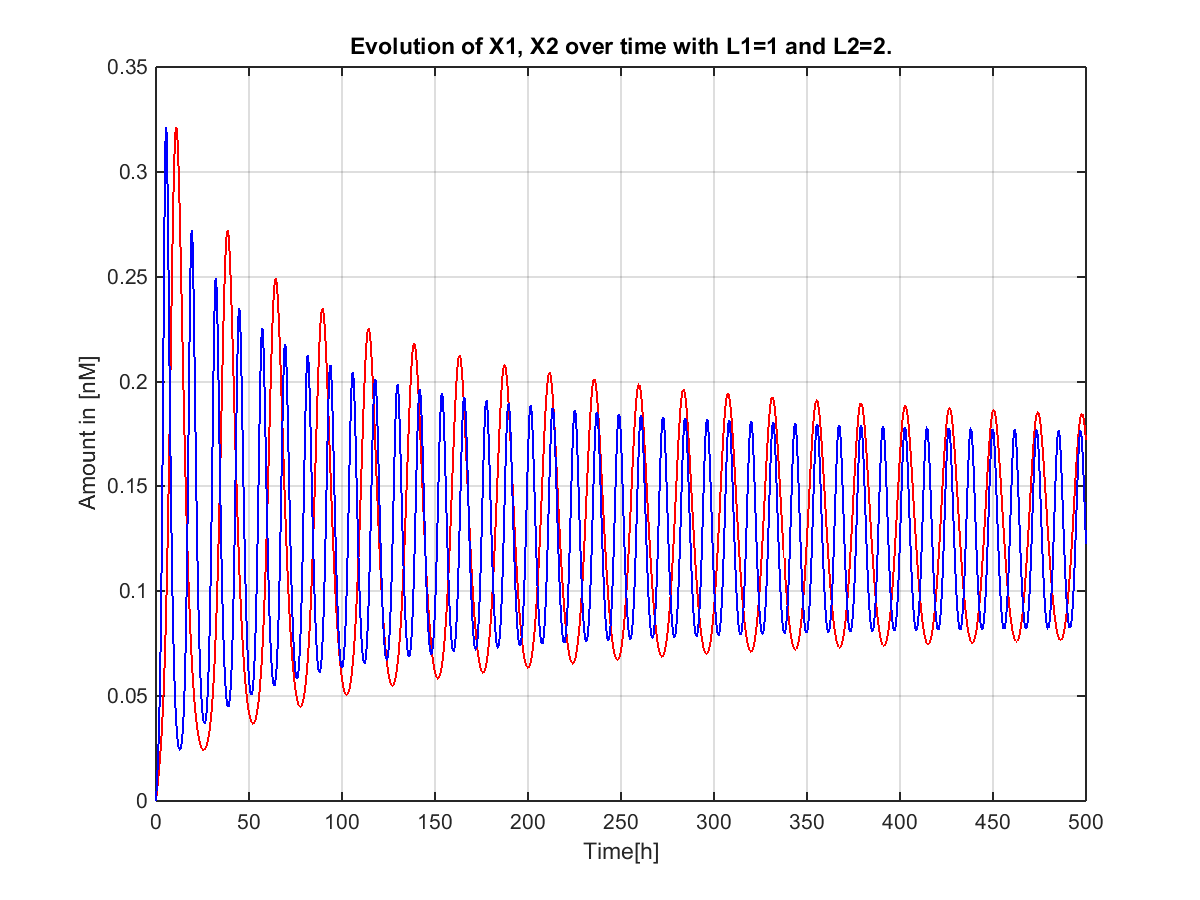
\includegraphics[width=\textwidth]{"../Miniprojet 2.0/Part B/B_2_graphs/B26.png}
	    \caption{$\lambda_1$ = 1, $\lambda_2$ = 2 [$h^{-1}$]}
	\end{subfigure}

	\caption{\red{$X_1(t)$} and \blue{$X_2(t)$} trajectories in a two-cells Model \\
	We observe that }
    \end{figure*}

    \begin{figure*}
    \centering
	\begin{subfigure}[b]{0.32\textwidth}
	    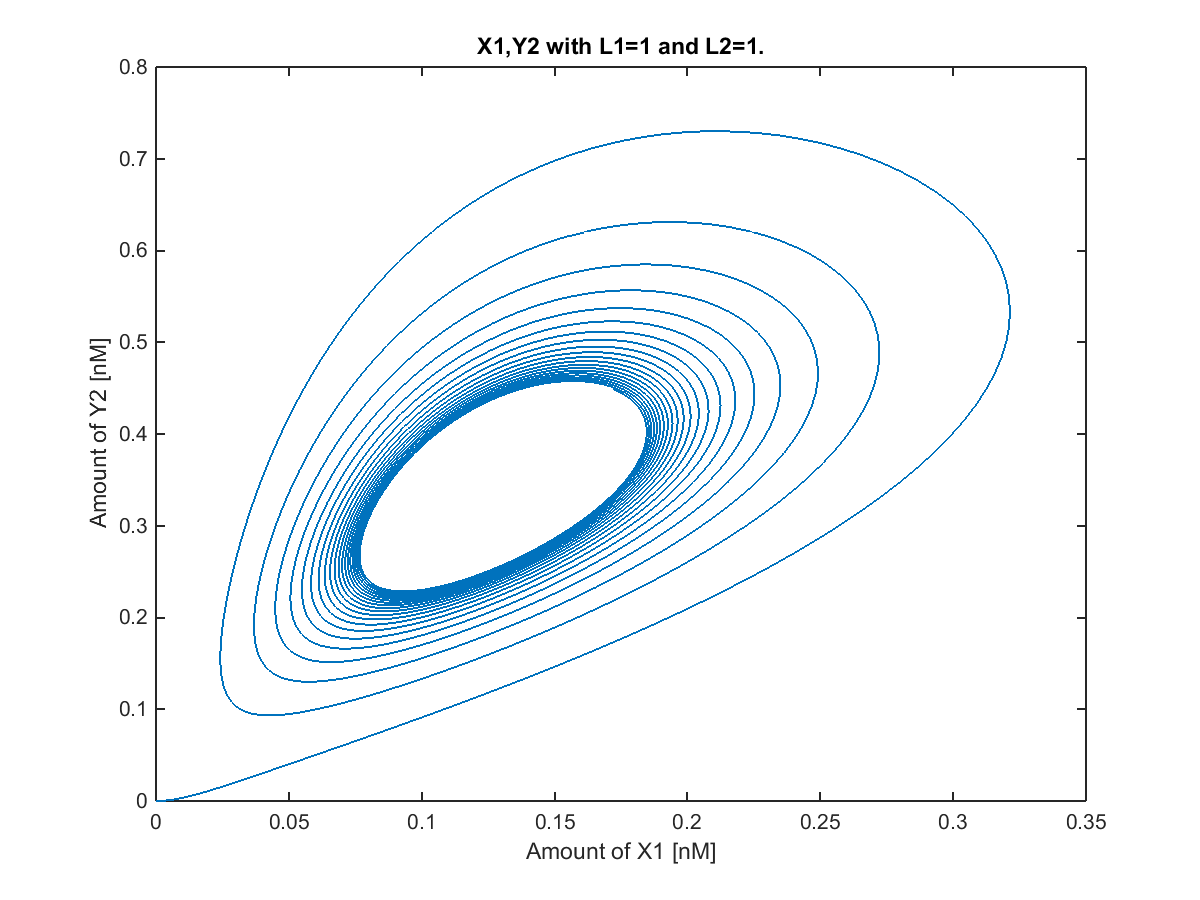
\includegraphics[width=\textwidth]{"../Miniprojet 2.0/Part B/B_2_graphs/B31.png}
	    \caption{$\lambda_1$ = 1, $\lambda_2$ = 1 [$h^{-1}$]}
	\end{subfigure}
	~ 
	\begin{subfigure}[b]{0.32\textwidth}
	    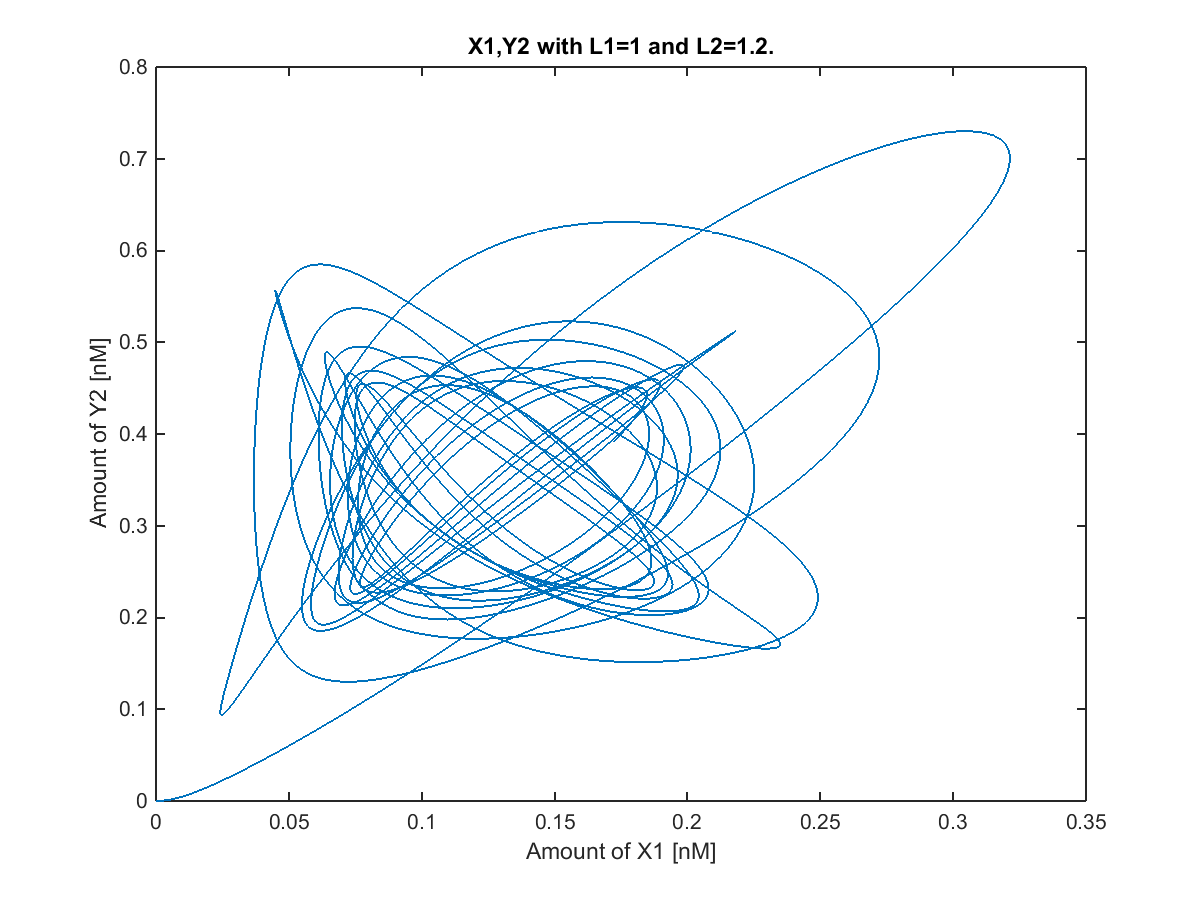
\includegraphics[width=\textwidth]{"../Miniprojet 2.0/Part B/B_2_graphs/B32.png}
	    \caption{$\lambda_1$ = 1, $\lambda_2$ = 1.2 [$h^{-1}$]}
	\end{subfigure}
	~ 
	\begin{subfigure}[b]{0.32\textwidth}
	    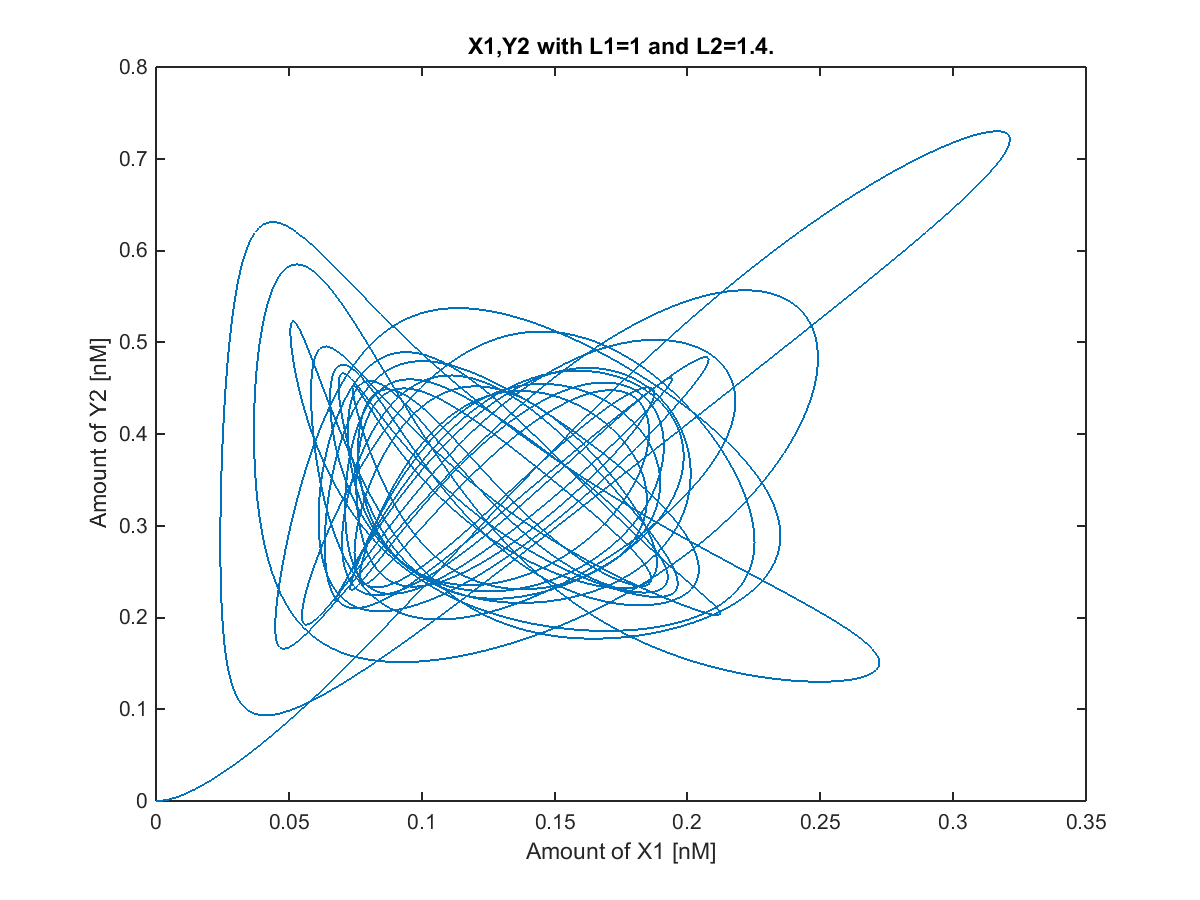
\includegraphics[width=\textwidth]{"../Miniprojet 2.0/Part B/B_2_graphs/B33.png}
	    \caption{$\lambda_1$ = 1, $\lambda_2$ = 1.4 [$h^{-1}$]}
	\end{subfigure}
	 
	\begin{subfigure}[b]{0.32\textwidth}
	    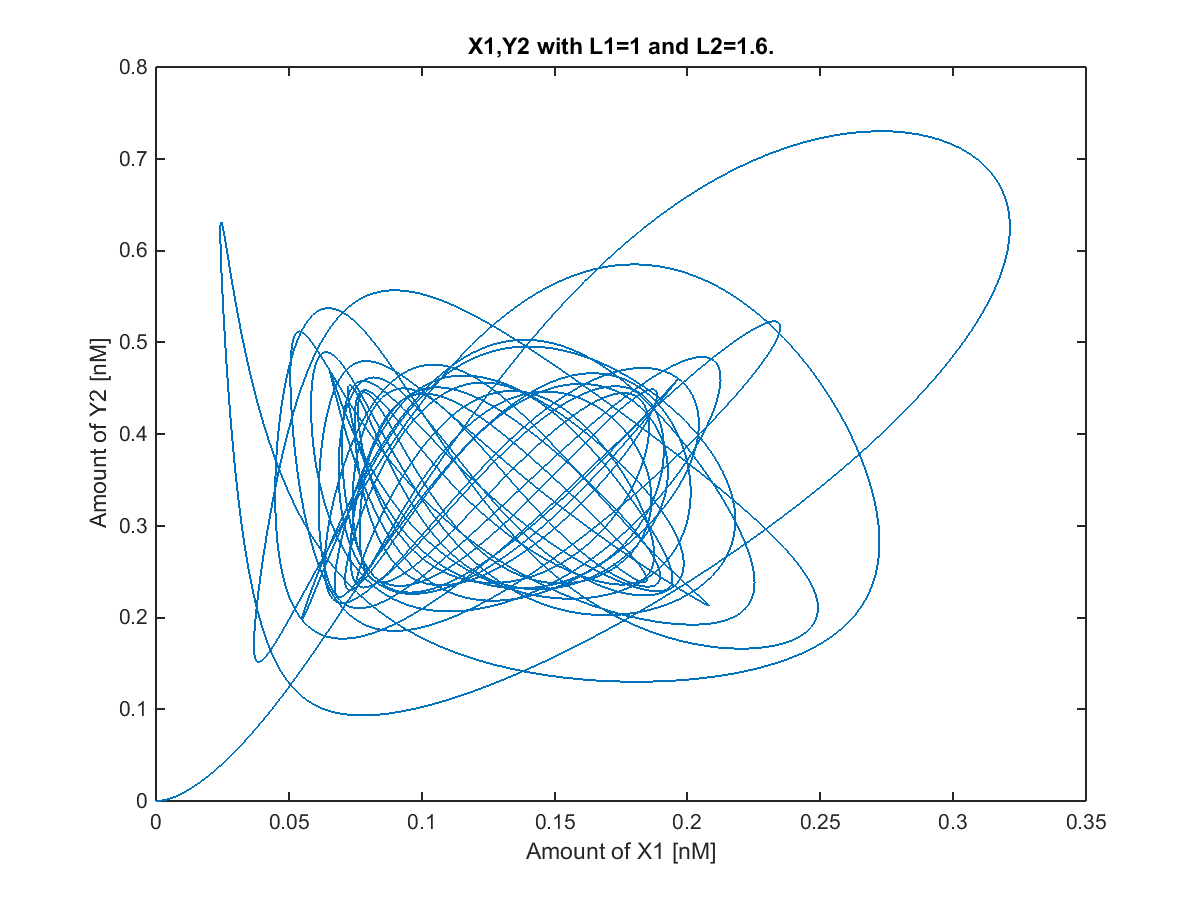
\includegraphics[width=\textwidth]{"../Miniprojet 2.0/Part B/B_2_graphs/B34.png}
	    \caption{$\lambda_1$ = 1, $\lambda_2$ = 1.6 [$h^{-1}$]}
	\end{subfigure}
	~ 
	\begin{subfigure}[b]{0.32\textwidth}
	    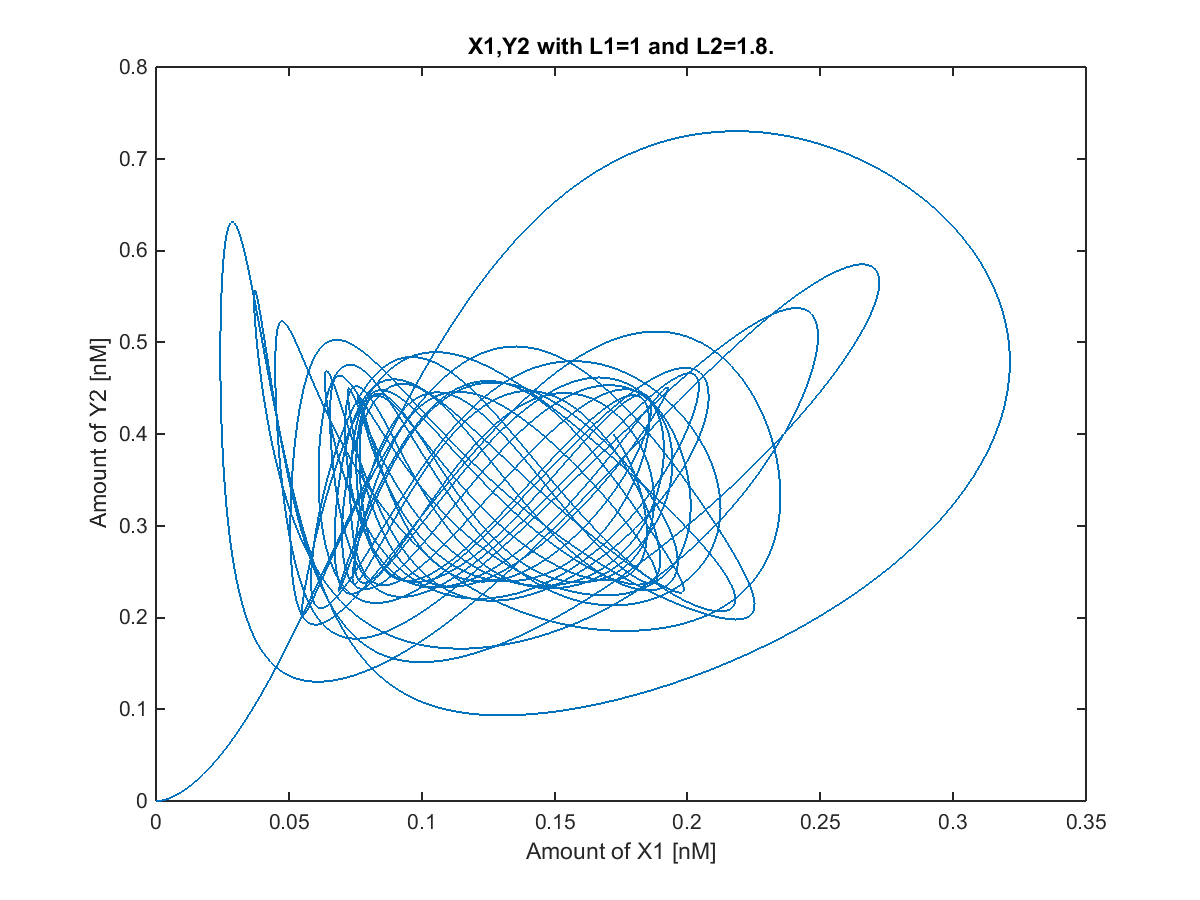
\includegraphics[width=\textwidth]{"../Miniprojet 2.0/Part B/B_2_graphs/B35.png}
	    \caption{$\lambda_1$ = 1, $\lambda_2$ = 1.8 [$h^{-1}$]}
	\end{subfigure}
	~ 
	\begin{subfigure}[b]{0.32\textwidth}
	    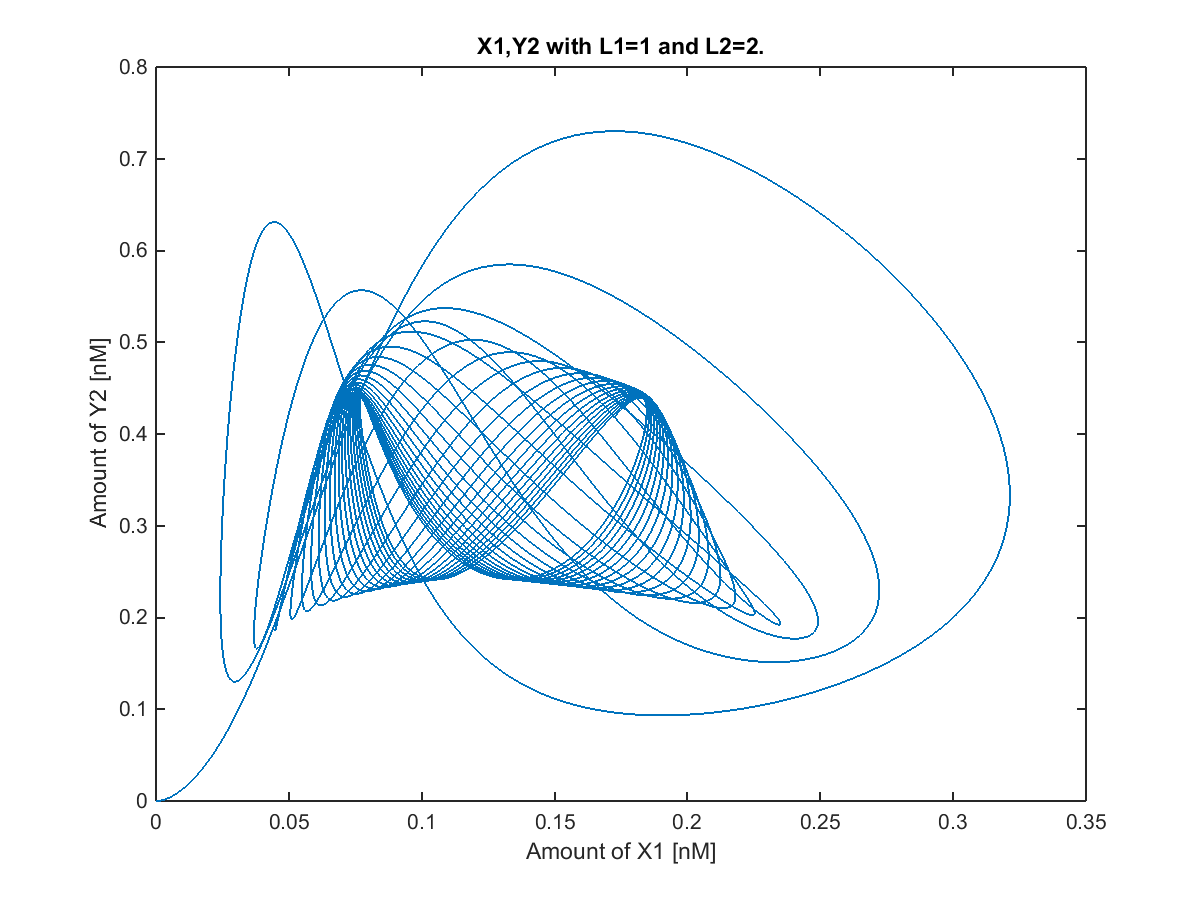
\includegraphics[width=\textwidth]{"../Miniprojet 2.0/Part B/B_2_graphs/B36.png}
	    \caption{$\lambda_1$ = 1, $\lambda_2$ = 2 [$h^{-1}$]}
	\end{subfigure}

	\caption{$X_1$ and $Y_2$ trajectories \\
	}
    \end{figure*}

    \begin{figure*}
    \centering
	\begin{subfigure}[b]{0.32\textwidth}
	    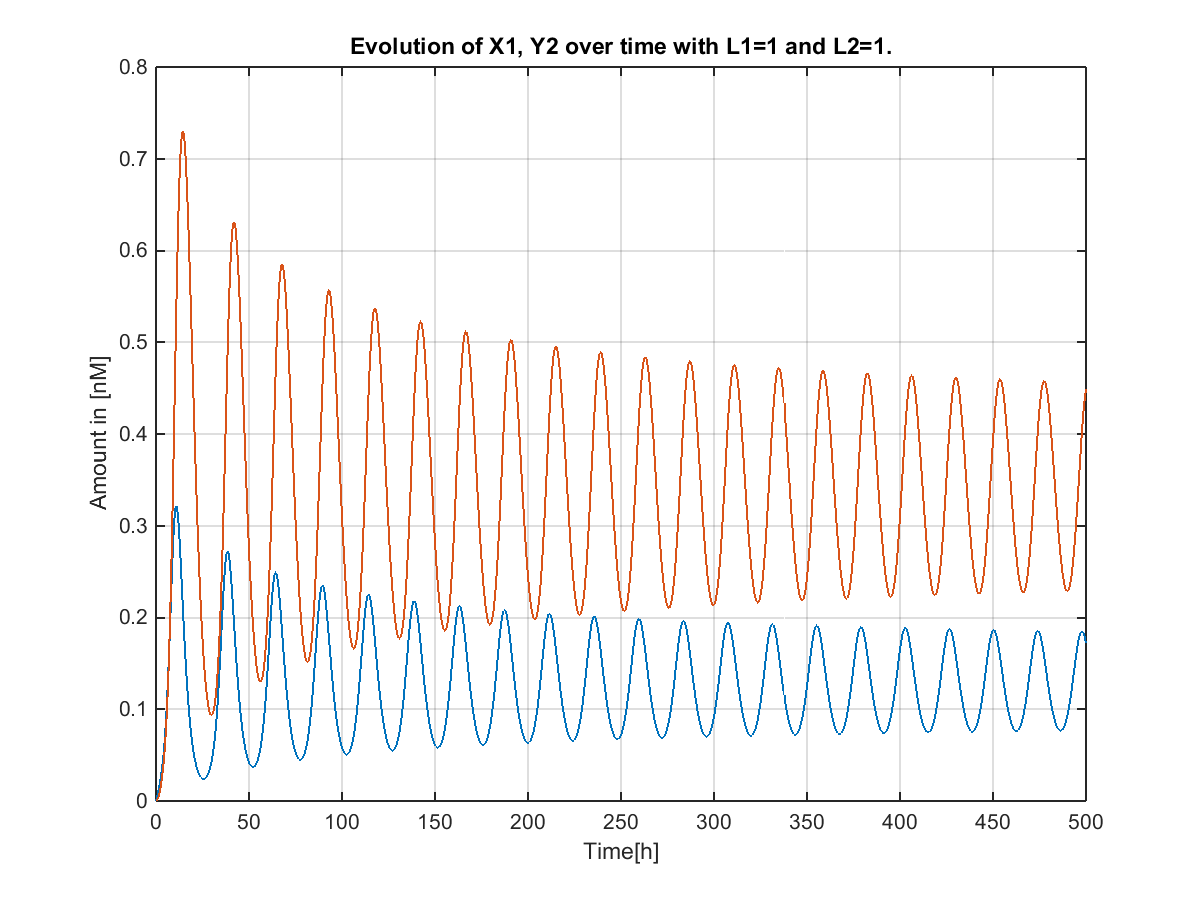
\includegraphics[width=\textwidth]{"../Miniprojet 2.0/Part B/B_2_graphs/B41.png}
	    \caption{$\lambda_1$ = 1, $\lambda_2$ = 1 [$h^{-1}$]}
	\end{subfigure}
	~ 
	\begin{subfigure}[b]{0.32\textwidth}
	    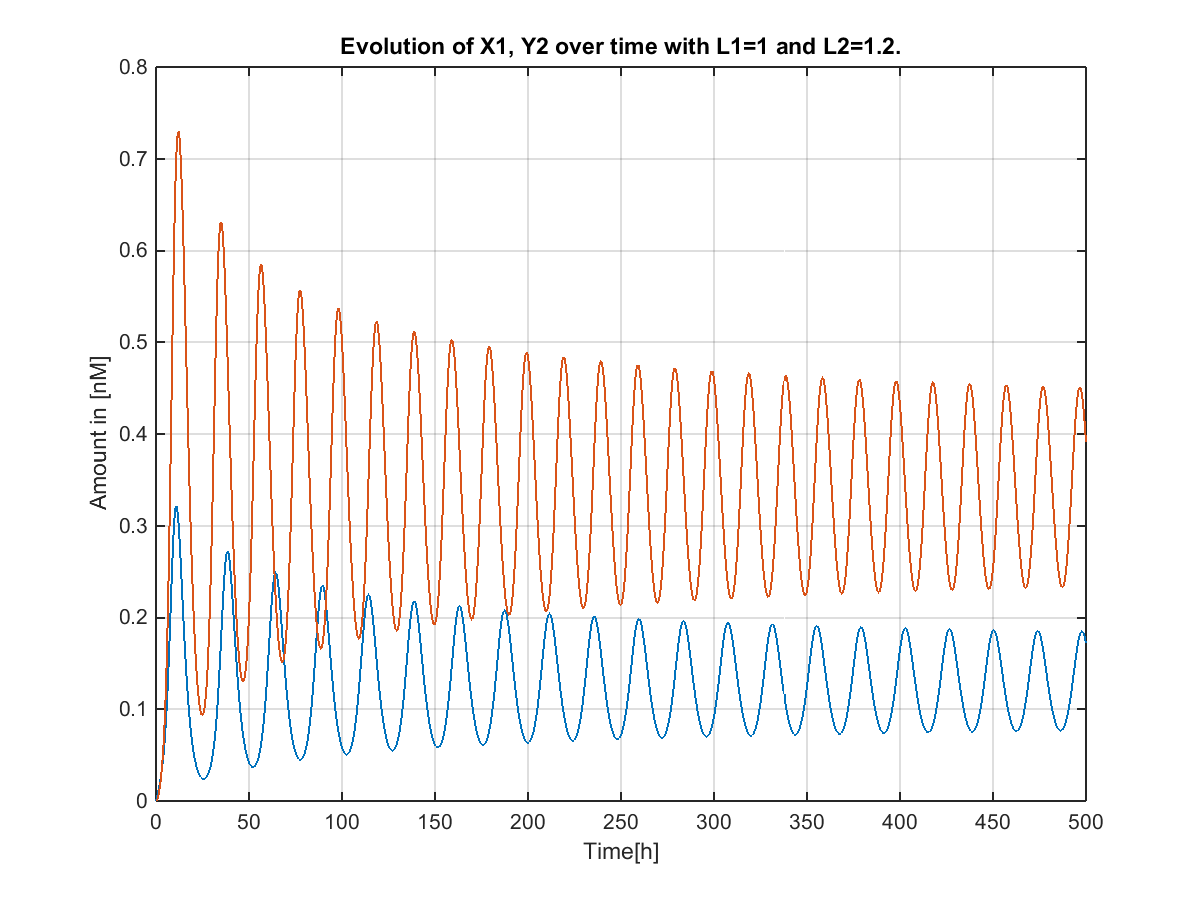
\includegraphics[width=\textwidth]{"../Miniprojet 2.0/Part B/B_2_graphs/B42.png}
	    \caption{$\lambda_1$ = 1, $\lambda_2$ = 1.2 [$h^{-1}$]}
	\end{subfigure}
	~ 
	\begin{subfigure}[b]{0.32\textwidth}
	    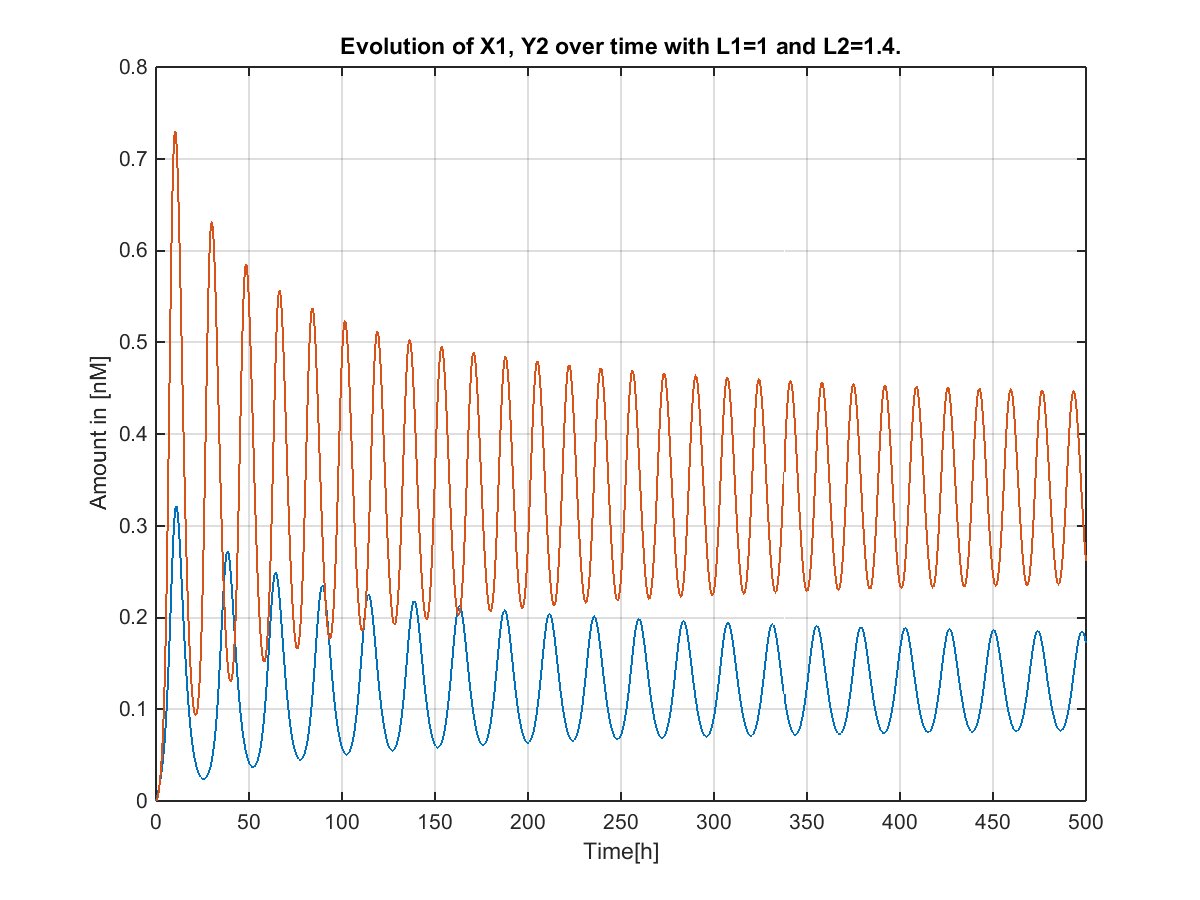
\includegraphics[width=\textwidth]{"../Miniprojet 2.0/Part B/B_2_graphs/B43.png}
	    \caption{$\lambda_1$ = 1, $\lambda_2$ = 1.4 [$h^{-1}$]}
	\end{subfigure}
	 
	\begin{subfigure}[b]{0.32\textwidth}
	    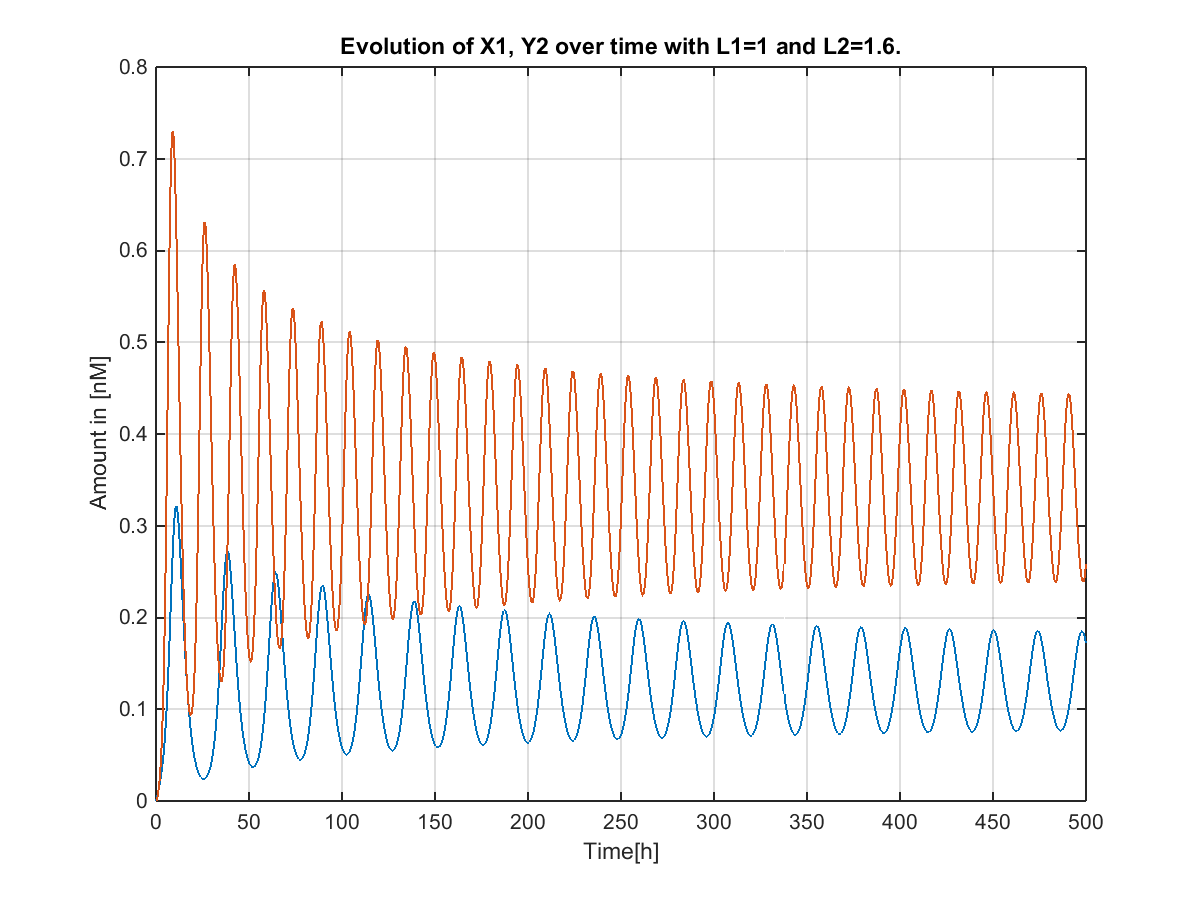
\includegraphics[width=\textwidth]{"../Miniprojet 2.0/Part B/B_2_graphs/B44.png}
	    \caption{$\lambda_1$ = 1, $\lambda_2$ = 1.6 [$h^{-1}$]}
	\end{subfigure}
	~ 
	\begin{subfigure}[b]{0.32\textwidth}
	    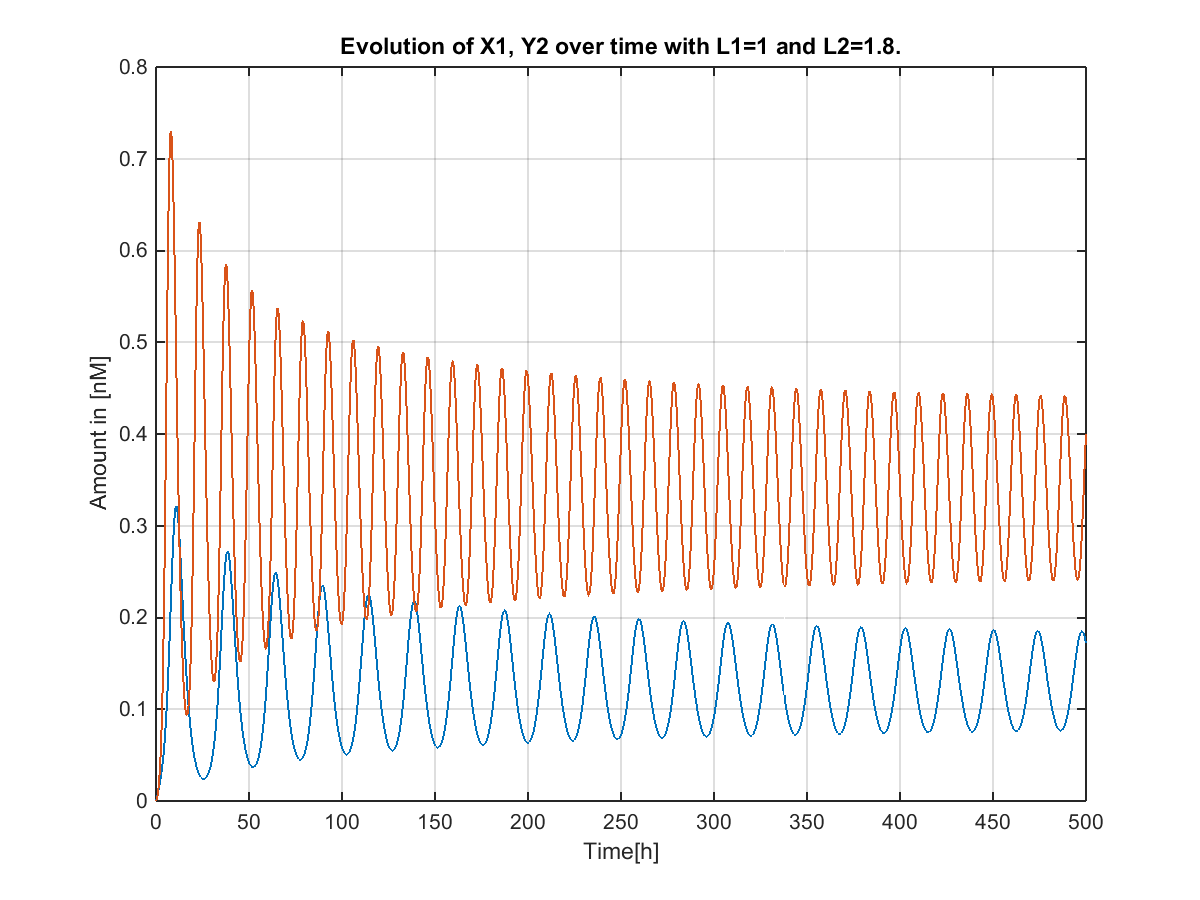
\includegraphics[width=\textwidth]{"../Miniprojet 2.0/Part B/B_2_graphs/B45.png}
	    \caption{$\lambda_1$ = 1, $\lambda_2$ = 1.8 [$h^{-1}$]}
	\end{subfigure}
	~ 
	\begin{subfigure}[b]{0.32\textwidth}
	    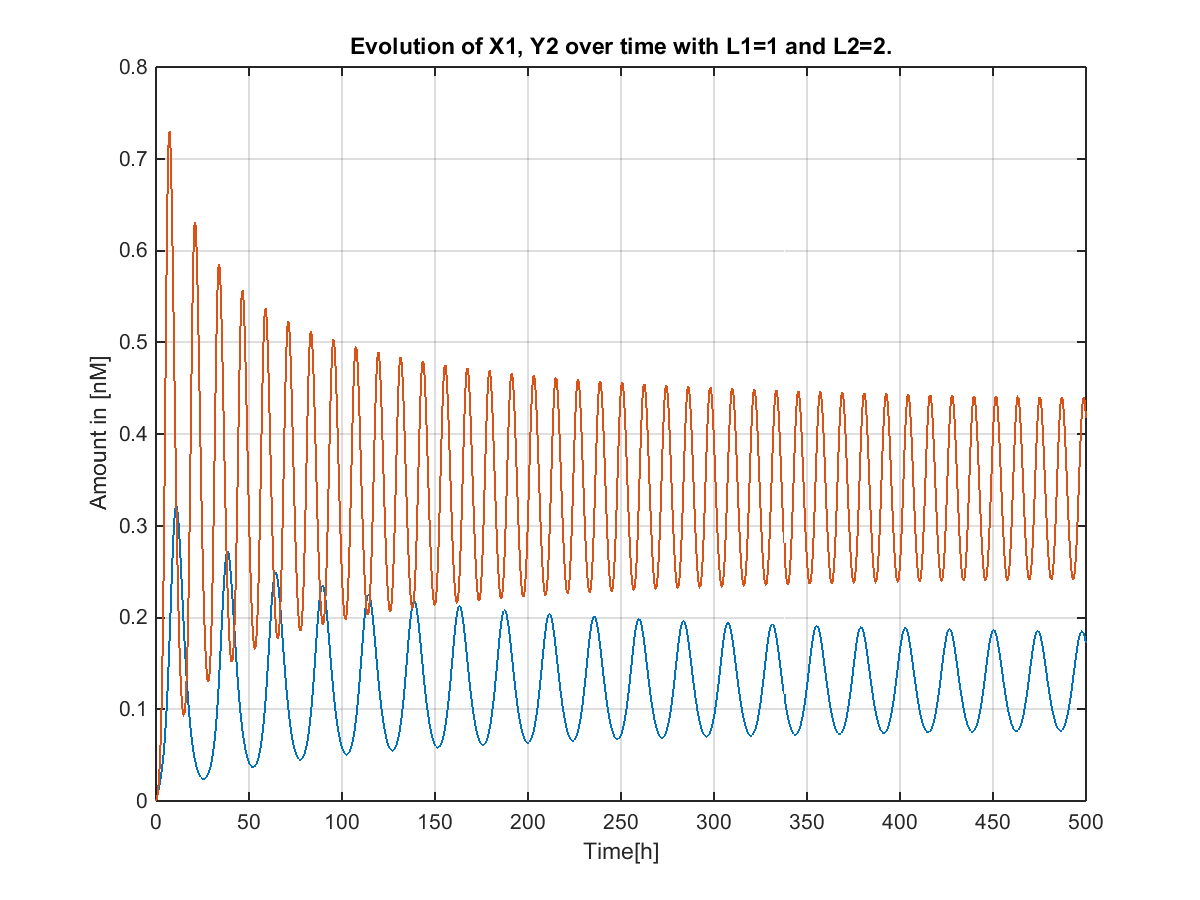
\includegraphics[width=\textwidth]{"../Miniprojet 2.0/Part B/B_2_graphs/B46.png}
	    \caption{$\lambda_1$ = 1, $\lambda_2$ = 2 [$h^{-1}$]}
	\end{subfigure}

	\caption{raraara}
    \end{figure*}

    \begin{figure*}
    \centering
	\begin{subfigure}[b]{0.45\textwidth}
	    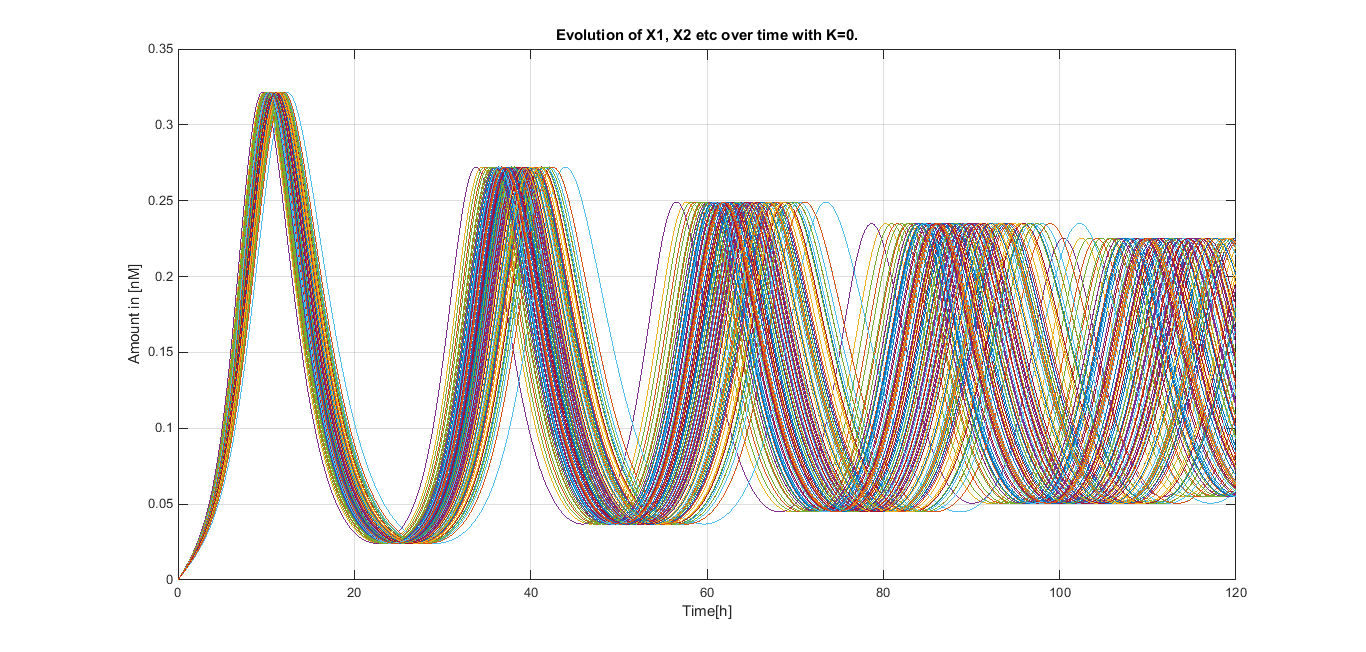
\includegraphics[width=\textwidth]{"../Miniprojet 2.0/Part B/100cells/100cells0_0.png}
	    \caption{$K=0.0$}
	\end{subfigure}
	~ 
	\begin{subfigure}[b]{0.45\textwidth}
	    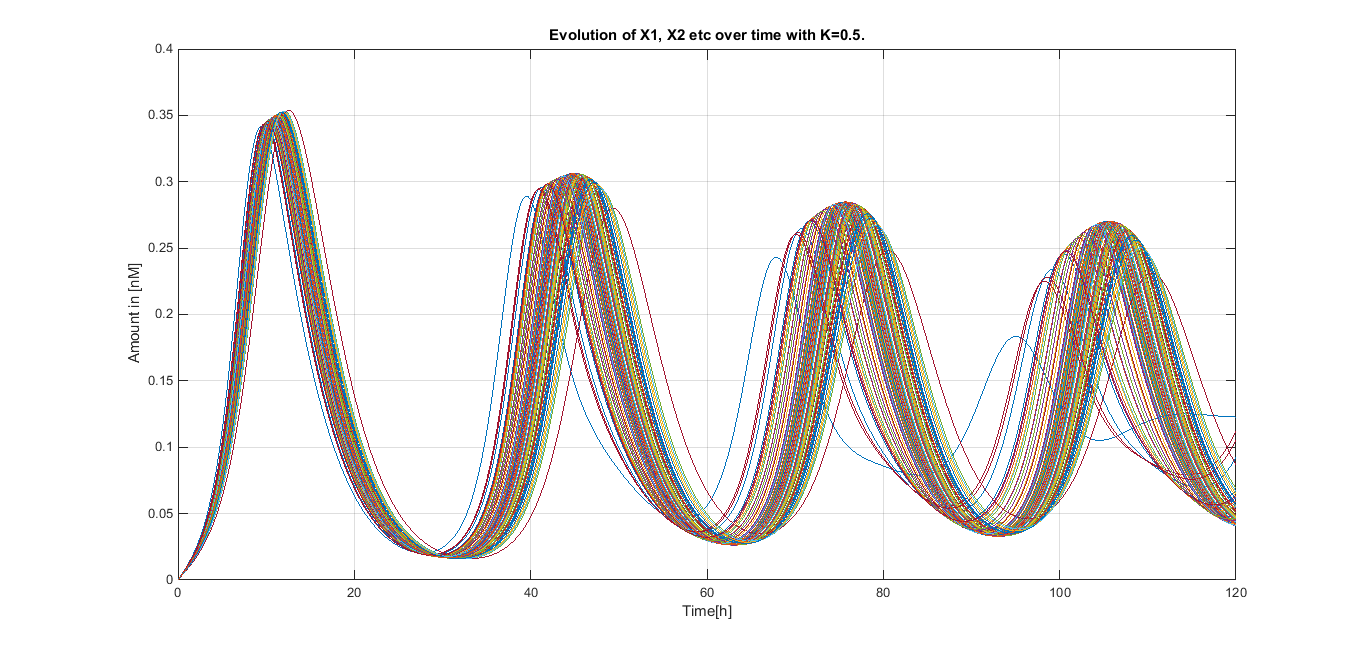
\includegraphics[width=\textwidth]{"../Miniprojet 2.0/Part B/100cells/100cells0_5.png}
	    \caption{$K=0.5$}
	\end{subfigure}
	~ 
	\begin{subfigure}[b]{0.45\textwidth}
	    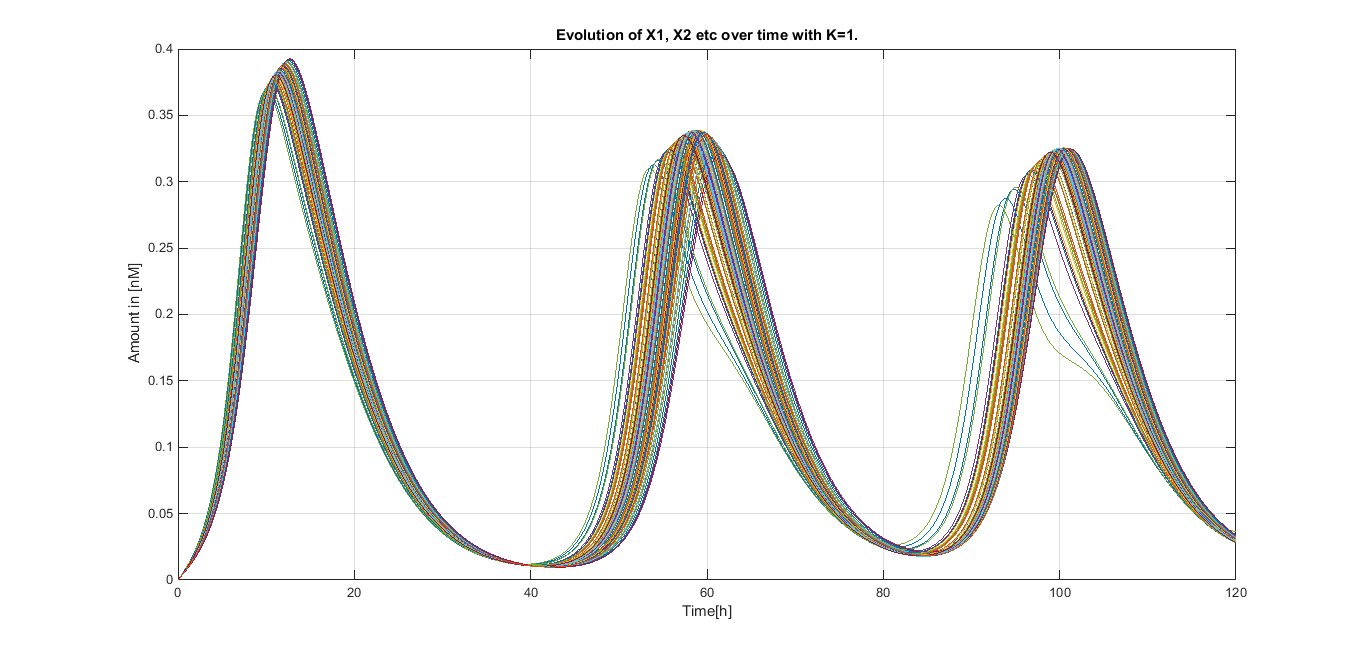
\includegraphics[width=\textwidth]{"../Miniprojet 2.0/Part B/100cells/100cells1_0.png}
	    \caption{$K=1.0$}
	\end{subfigure}
	 
	\begin{subfigure}[b]{0.45\textwidth}
	    \includegraphics[width=\textwidth]{"../Miniprojet 2.0/Part B/100cells/100cells1_5a.png}
	    \caption{$K=1.5$}
	\end{subfigure}
	~ 
	\begin{subfigure}[b]{0.45\textwidth}
	    \includegraphics[width=\textwidth]{"../Miniprojet 2.0/Part B/100cells/100cells1_5b.png}
	    \caption{$K=1.5$}
	\end{subfigure}

	\caption{raraara}
    \end{figure*}

    \begin{figure*}
    \centering
	\begin{subfigure}[b]{0.3\textwidth}
	    \includegraphics[width=\textwidth]{"../Miniprojet 2.0/Part B/B_3_bifurcation.png}
	    \caption{$K=0.0$}
	\end{subfigure}
	~ 
	\begin{subfigure}[b]{0.3\textwidth}
	    \includegraphics[width=\textwidth]{"../Miniprojet 2.0/Part B/B_3_bifurcation_2.png}
	    \caption{$K=0.3$}
	\end{subfigure}
	~ 
	\begin{subfigure}[b]{0.3\textwidth}
	    \includegraphics[width=\textwidth]{"../Miniprojet 2.0/Part B/B_N_3_graph_2.png}
	    \caption{$K=1.0$}
	\end{subfigure}
	\caption{raraara}
    \end{figure*}


\end{document}
